\documentclass[oneside,12t]{classes/Thesis}

\usepackage[utf8]{inputenc}
\usepackage{ulem}
\usepackage[english]{babel}

\usepackage{url}
\graphicspath{{img/},{resultat_rostand/},{resultat_manumanu/}}
\DeclareGraphicsExtensions{.pdf,.png}

\usepackage[T1]{fontenc}
\usepackage{pslatex}

\usepackage{fixltx2e}


\usepackage[french,onelanguage,ruled]{algorithm2e}
%\usepackage{algorithmic}
\usepackage{caption}
\usepackage{subfigure}

\usepackage{color}
\usepackage{listingsutf8}

%listings}

\definecolor{cppred}{rgb}{0.6,0,0} % for strings
\definecolor{cppgreen}{rgb}{0.25,0.5,0.35} % comments
\definecolor{cpppurple}{rgb}{0.5,0,0.35} % keywords
\definecolor{cppblue}{rgb}{0.25,0.35,0.75} % javadoc

\lstset{
  language=C++,
  numbers=left,
  numberstyle=\footnotesize,
  stepnumber=1,
  backgroundcolor=\color{white},
  identifierstyle=\color{cpppurple},
  keywordstyle=\bfseries,
  stringstyle=\color{cppred},
  commentstyle=\color{cppgreen},
  showspaces=false,
  showstringspaces=false,
  showtabs=false,
  frame=single,
  tabsize=2,
  captionpos=b,
  breaklines=true,
  breakatwhitespace=false,
  escapeinside={\%*}{*)}
}





\title{Un modèle de programmation à grain fin pour la parallélisation de solveurs linéaire creux}


\authorFirstName{Corentin}
\authorLastName{Rossignon}
\authorMail{corentin.rossignon@gmail.com}

\directors{Raymond \textsc{Namyst}}
\codirectors{Olivier \textsc{Aumage} et Samuel \textsc{Thibault}}
\responsables{Pascal \textsc{H\'{e}non}}

\laboratory{LaBRI}
\laboratoryURL{http://www.labri.fr/}
\university{Université de Bordeaux}
\universityURL{http://www.univ-bordeaux.fr/}


\logo{bordeaux1}
\degreeDate{?? ???? 2015}
\degree{Docteur de l'université de Bordeaux}
\degreeSpeciality{Informatique}

\metadataSetup

% turn of those nasty overfull and underfull hboxes
\hbadness=10000
\hfuzz=50pt

\begin{document}

\dominitoc
\tikzstyle{decision} = [diamond, draw, fill=blue!20,
text width=3em, text centered, node distance=2.5cm, inner sep=0pt,font=\scriptsize]
\tikzstyle{block} = [rectangle, draw, fill=blue!20,
text width=4em, text centered, rounded corners, minimum height=1em,font=\scriptsize]
\tikzstyle{line} = [draw, thick, color=black!50,font=\scriptsize]
\tikzstyle{cloud} = [draw, ellipse,fill=red!20, node distance=2.5cm,
minimum height=0.1em,font=\scriptsize]

\maketitle

%set the number of sectioning levels that get number and appear in the contents
\setcounter{secnumdepth}{3}
\setcounter{tocdepth}{3}

\frontmatter % book mode only
\pagenumbering{roman}
%\input{src/acknowledgement}
%La résolution de grands systèmes linéaire creux est un élément essentiel des simulations numériques. Ces résolutions peuvent représenter jusqu'à 80\% du temps de calcul des simulations.
Une parallélisation efficace des noyaux d'algèbre linéaire creuse conduira donc à obtenir de meilleurs performances. En mémoire distribuée, la parallélisation de ces noyaux se fait le plus souvent en modifiant le schéma numérique. Par contre, en mémoire partagée, un parallélisme plus efficace peut être utilisé. Il est donc important d'utiliser deux niveaux de parallélisme, un premier niveau entre les noeuds d'une grappe de serveur et une deuxième niveau à l'intérieur du noeud. Lors de l'utilisation de méthodes itératives en mémoire partagée, les graphes de tâches permettent de décrire naturellement le parallélisme en prenant comme granularité le travail sur une ligne de la matrice. Malheureusement, cette granularité est trop fine et ne permet pas d'obtenir de bonnes performances.
Dans cette thèse, nous allons étudier le problème de la granularité pour la parallélisation par graphe de tâches. Nous proposerons d'augmenter la granularité des tâches de calcul en créant des agrégats de tâches qui deviendront eux-mêmes des tâches. L'ensemble de ces agrégats et des nouvelles dépendances entre les agrégats formera un graphe de granularité plus grossière. Ce graphe sera ensuite utilisé par un ordonnanceur de tâches pour obtenir de meilleurs résultats. Nous utiliserons comme exemple la factorisation ILU d'une matrice et nous montrerons les améliorations apportées par cette méthode. Dans un second temps, nous nous concentrerons sur les machines à architecture NUMA. Dans le cas de l'utilisation d'algorithmes limités par la bande passante mémoire, il est intéressant de réduire les effets NUMA liés à cette architecture. Nous montrerons comment prendre en compte ces effets dans un intergiciel à base de tâches pour améliorer les performances d'un programme.

Mots-clés : parallélisme, graphe de tâches, supports d’exécution, NUMA, multi-coeurs, algèbre linéaire creuse

%Solving large sparse linear system is an essential part of numerical simulations. These resolve can take up to 80\% of the total of the simulation time.
An efficient parallélization of sparse linear kernels inéaire creuse leads to obtain better performances. In distributed memory, parallélization of theses kernels are often done by changing the numerical scheme. Par contreContrariwise, in shared memory, a more efficient parallelism can be used. It's significant to use two levels of parallelism, a first one between nodes of a cluster and a second inside a node. Lors de l'utilisation de méthodes itératives en mémoire partagée, les graphes de tâches permettent de décrire naturellement le parallélisme en prenant comme granularité le travail sur une ligne de la matrice. Malheureusement, cette granularité est trop fine et ne permet pas d'obtenir de bonnes performances.
Dans cette thèse, nous allons étudier le problème de la granularité pour la parallélisation par graphe de tâches. Nous proposerons d'augmenter la granularité des tâches de calcul en créant des agrégats de tâches qui deviendront eux-mêmes des tâches. L'ensemble de ces agrégats et des nouvelles dépendances entre les agrégats formera un graphe de granularité plus grossière. Ce graphe sera ensuite utilisé par un ordonnanceur de tâches pour obtenir de meilleurs résultats. Nous utiliserons comme exemple la factorisation ILU d'une matrice et nous montrerons les améliorations apportées par cette méthode. Dans un second temps, nous nous concentrerons sur les machines à architecture NUMA. Dans le cas de l'utilisation d'algorithmes limités par la bande passante mémoire, il est intéressant de réduire les effets NUMA liés à cette architecture. Nous montrerons comment prendre en compte ces effets dans un intergiciel à base de tâches pour améliorer les performances d'un programme.

Mots-clés : parallélisme, graphe de tâches, supports d’exécution, NUMA, multi-coeurs, algèbre linéaire creuse

\tableofcontents
\mtcaddchapter
\mainmatter % book mode only



%=========================================================
\chapter{Contexte : simuler l'extraction du pétrole}
\minitoc
\vspace{1cm}
%=========================================================

%+++++++++++++++++++++++++++++++
\section{La simulation de réservoir}
%-------------------------------
\subsection{Overview}

%
Into the depth of the Earth, petroleum and natural gas are trapped.
%
These sources of energy are the result of the transformation of organic matter coming from vegetables and dead animals under very high constraint during millions of years.
%
Hardly hide under several kilometers of stone, petroleum companies, as Total S.A., tried to find them all, before a concurrent company.



More generally, we call reservoir of hydrocarbon, or shorter just reservoir, a major concentration of petroleum and/or natural gas under the ground.
%
The first step to find a reservoir is to analyze the underground with seismic waves.
%
These waves are generated by bomb for under sea analysis or with seismic truck for the surface of the Earth.
%
When these seismic waves are analyzed with some waves equation modeling software, petroleum companies can obtain a pretty good representation of the underground.
%
When a reservoir is found, one of the first questions is : "Does it pay to exploit this reservoir ?".
%
Reservoir simulations help to answer this question.
%
By doing a flow of fluid simulation through porous media, petroleum companies can obtain an approximation of the among of possible oil recovering.
%
If it is profitable to exploit the reservoir, petroleum companies can start exploiting the reservoir.



But it is not sufficient to dig and wait for petroleum sprung in a geyser form like we can see in animated cartoon.
%
Petroleum companies need to install some wells.
%
There are two major kinds of wells (Fig .\ref{fig:wells}) :
%
\begin{itemize}
  \item Injector wells, this is the wells which will increase pressure inside the reservoir by injecting matter (water, polymer, ..).
  \item Production wells, this is the wells which will recovery oil, they are also essential to control pressure by producing more or less oil.
\end{itemize}

%   (-_-)   %
\begin{figure}[!ht]
  \centering
  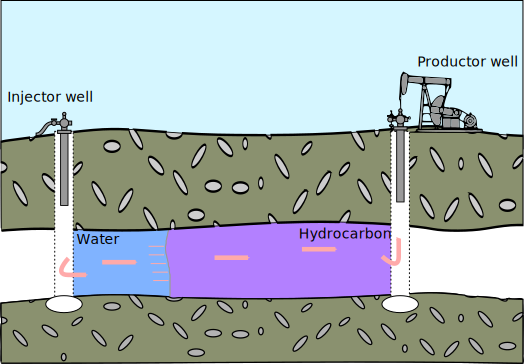
\includegraphics[width=0.8\textwidth]{wells}
  \caption{An oil field with two wells.}
\label{fig:wells}
\end{figure}


Reservoir engineers need to find the optimal number of wells and also their optimal placement.
%
Again, they use reservoir simulations to test different configurations.
%
Later, when the petroleum company starts exploiting the field, it can be interesting to forecast oil production.
%
Once again, reservoir simulation helps (Fig. \ref{fig:floviz}).

%   (-_-)   %
\begin{figure}[!ht]
  \centering
  \includegraphics[width=\textwidth]{reservoir}
  \caption{Saturation of oil in a reservoir during a simulation.}
\label{fig:floviz}
\end{figure}


As shown previously, reservoir simulation is a key step in the oil recovery process.
%
Petroleum companies want to simulate more and more precisely internal state of a reservoir, and of course as quickly as possible.
%
Let's see the structure of a reservoir simulator.

%-------------------------------
\subsection{From physics to computation}
To be able to do reservoir simulation, we start with a physicist who model fluid flow inside porous medium.
%
From this model, we can obtain some physical equations.
%
Then we discretize the reservoir into cells and we use a finite difference schema.
%
For each cell of the reservoir, we can compute a non-linear equation of each variables (e.g.: pressure, oil saturation)
%
To solve the non-linear systems of equation, we use the Newton–Raphson method.
%
This method is iterative, we begins with an initial guess $X_0$ reasonably close to the solution $X_n$ which satisfied $F(X_n) = 0$.

%   (-_-)   %
\begin{figure}[!ht]
  \centering
  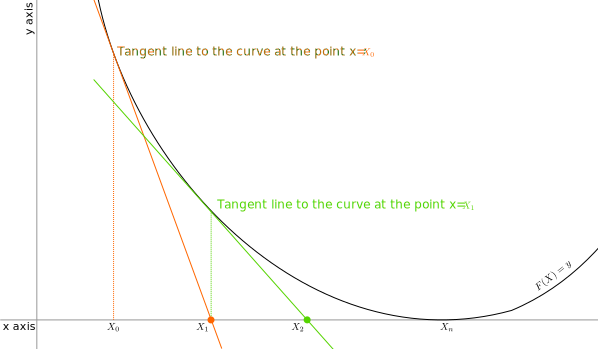
\includegraphics[width=\textwidth]{newton}
  \caption{Example of two Newton steps in one dimension space.
    Each tangent lines correspond to a linear equation to solve.}
\label{newton}
\end{figure}

The example in the figure~\ref{newton} is only in one dimension but it's quite the same approach that can be done when we work with an arbitrary number of dimensions.
%
Linear equations of reservoir siluation can be represent as large sparse matrices.
%
Each row represent all interactions between an element and its direct neighbors.
%
So in a regular mesh, there can have up to seven small dense block per row.
%
Sparse linear algebra solvers, like GMRES, are then utilize to solve all linear problems use in the Newton method.
%
Let's focus on linear algebra.

%-------------------------------
\subsection{Simulation of a simple physical example}
Let's take a simple physical example to see how linear algebra can be used in physical simulation.
%
We want to simulate the pressure of an oil column.
%
We know that the density of the oil presents in the column is $\rho = 0.9192~kg/m^3$.
%
We also know the physical equation of the hydrostatic pressure:
%
\begin{equation}
\label{eq:hydrostatic}
\frac{\mathrm d P}{\mathrm d z} = \rho{}g
\end{equation}
%
where $P$ is the pressure, $z$ is the depth and $g$ is the gravitational acceleration.
%
By using the Taylor's theorem at first order, we obtain the equation:
%
\begin{equation}
P(z_0+h) = P(z_0) + h \frac{\mathrm d P}{\mathrm d z} (z_0) + o(h^2)
\end{equation}
\begin{equation}
\frac{\mathrm d P}{\mathrm d z} (z_0) = \frac{P(z_0+h) - P(z_0)}{h} + o(h^2)
\end{equation}

%   (-_-)   %
\begin{figure}[!ht]
  \centering
  \includegraphics[width=0.5\textwidth]{rocks}
  \caption{oil column scheme.}
  \label{fig:oil_schema}
\end{figure}
%
We discretize the problem in $n$ cells with a finite difference method (fig.~\ref{fig:oil_schema}): let us consider $Z_i$ the approximation of $z$ on the cell $i$, $i$ going from $0$ to $n-1$.
%
Each cells are separate by a distance $h$ called $\Delta{z}$:
%
\begin{equation}
\label{eq:taylor_fd}
\frac{\mathrm d P}{\mathrm d z}(Z_i) \approx \frac{P(Z_{i}) - P(Z_{i-1})}{\Delta{z}}
\end{equation}
%
By injecting \eqref{eq:taylor_fd} in \eqref{eq:hydrostatic} leads to:
%
\begin{equation}
\frac{P(Z_{i}) - P(Z_{i-1})}{\Delta{z}} = \rho{}g
\end{equation}
\begin{equation}
\label{eq:system_pressure}
P(Z_{i}) - P(Z_{i-1}) = \rho{}g\Delta{z}
\end{equation}
We also have the boundary condition that at ground level 0, the pressure is 1000~hPa or $10^5$~Pa:
%
\begin{equation}
P(Z_0) = 10^5
\end{equation}
%
We can now write the entire system under a matrix form with $n$ cells:
%
\begin{equation}
\label{eq:ax_b}
\begin{bmatrix}
   1   &    0   &    0   & \cdots & \cdots & \cdots & \cdots &   0    \\
  -1   &    1   &    0   & \ddots &        &        &        & \vdots \\
   0   &   -1   &    1   &    0   & \ddots &        &        & \vdots \\
\vdots & \ddots & \ddots & \ddots & \ddots & \ddots &        & \vdots \\
\vdots &        & \ddots & \ddots & \ddots & \ddots & \ddots & \vdots \\
\vdots &        &        & \ddots &   -1   &    1   &    0   &   0    \\
\vdots &        &        &        & \ddots &   -1   &    1   &   0    \\
   0   & \cdots & \cdots & \cdots & \cdots &    0   &   -1   &   1    \\
\end{bmatrix}
\begin{pmatrix}
  P(Z_0)  \\
  P(Z_1)  \\
\vdots \\
\vdots \\
\vdots \\
\vdots \\
P(Z_{n-2}) \\
  P(Z_{n-1})  \\
\end{pmatrix}
=
\begin{pmatrix}
 10^5  \\
\rho{}g\Delta{z}     \\
\vdots \\
\vdots \\
\vdots \\
\vdots \\
\rho{}g\Delta{z} \\
\rho{}g\Delta{z}    \\
\end{pmatrix}
\end{equation}
By doing the multiplication of each line of $A$ by $x$, we obtain exactly the system of equations \eqref{eq:system_pressure}.
%
Now, we have a matrix $A$ multiply a vector $x$ equal a vector $b$, it's time to talk about linear algebra.

%+++++++++++++++++++++++++++++++


%+++++++++++++++++++++++++++++++
\section{Algèbre linéaire}
%-------------------------------
\subsection{Dense linear algebra}

Let's take a real life example to see what linear algebra is and how to use it.
%
We need to simulate the pressure of the underground which contains three different rocks.
%
Each rock has a density designed by $\rho$ and $rho(z)$ represents the density of the rock at the depth $z$.
%

%
We use the physical equation :
%
\begin{equation}
\frac{\mathrm d P}{\mathrm d z} = \rho(z)g
\end{equation}
%
where $P$ is the pressure, $z$ is the depth and $g$ is the gravitational constant.
%
We also have the boundary condition that at ground level 0, the pressure is 1000~hPa :
%
\begin{equation}
P_0 = 1000
\end{equation}
%
If we use a finite difference method at the first order
%
\begin{equation}
\frac{P_i - P_{i-1}}{z_i - z_{i-1}} = \rho(z_i)g
\end{equation}
%
If the distance between the center of all cells is the same, we can call it $\Delta{z}$ and we can replace $z_i - z_{i-1}$ by $\Delta{z}$ and multiply all terms by $\Delta{z}$ :
%
\begin{equation}
\label{eq:system_pressure}
P_i - P_{i-1} = \rho(z_i)g\Delta{z}
\end{equation}
%
\begin{equation}
\label{eq:ax_b}
\begin{bmatrix}
   1   &    0   &    0   & \cdots & \cdots & \cdots & \cdots &   0    \\
  -1   &    1   &    0   & \ddots &        &        &        & \vdots \\
   0   &   -1   &    1   &    0   & \ddots &        &        & \vdots \\
\vdots & \ddots & \ddots & \ddots & \ddots & \ddots &        & \vdots \\
\vdots &        & \ddots & \ddots & \ddots & \ddots & \ddots & \vdots \\
\vdots &        &        & \ddots &   -1   &    1   &    0   &   0    \\
\vdots &        &        &        & \ddots &   -1   &    1   &   0    \\
   0   & \cdots & \cdots & \cdots & \cdots &    0   &   -1   &   1    \\
\end{bmatrix}
*
\begin{pmatrix}
  P_0  \\
  P_1  \\
\vdots \\
\vdots \\
\vdots \\
\vdots \\
P_{i-1} \\
  p_i  \\
\end{pmatrix}
=
\begin{pmatrix}
 1000  \\
\rho(z_1)g\Delta{z}     \\
\vdots \\
\vdots \\
\vdots \\
\vdots \\
\rho(z_{i-1})g\Delta{z} \\
\rho(z_i)g\Delta{z}    \\
\end{pmatrix}
\end{equation}


We have a matrix $A$ multiply a vector $x$ equal a vector $b$.
%
By doing the multiplication we obtain exactly the system of equations \ref{eq:system_pressure}.
%
So solving a linear problem is often solving a problem of type $A*x=b$, many methods exist for solving this problem (Gaussian elimination, ...).
%
In this example, we already have a triangular matrix, so the solution can be found directly by solving each equation one-by-one starting with $P_0 = 1000$.


In computer science, there is a lot of library for doing linear algebra operations.
%
The most common is BLAS\footnote{Basic Linear Algebra Subprograms} which is a set of linear algebra operations.
%
These operations are classify into 3 categories :
\begin{itemize}
  \item Level 1 : it's vectors operations (dot products, addition of two vectors, ...)
  \item Level 2 : it's matrix-vector operations (multiply a matrix by a vector, solve a system of linear equations whose coefficients are in a triangular matrix, ...)
  \item Level 3 : it's matrix-matrix operations (multiply a matrix by a matrix, ...)
\end{itemize}
%
The level of BLAS is linked to the complexity in number of operations.
%
BLAS of Level 1 are bandwidth limited, there is no data reuse, each data is used only once.
%
BLAS of Level 2 can reuse vector data, some optimization can be done here.
%
BLAS of level 3 have a higher complexity and a lot of optimization exists.

Another library for library algebra is LAPACK\footnote{Linear Algebra PACKage}, it's build on top of BLAS.
%
Operations done by BLAS and LAPACK are well optimized, they have tilling optimization for cache blocking technique which improve data locality and reduce cache misses.
%
They also can use SIMD instructions(SSE, AVX, ...) in modern processor.
%
Some GPGPU versions also exist as well as versions for distributed memory.
%
Most of these optimizations can be done because the access pattern of BLAS operations are deterministic and some operations can be reorder without changing the final result.


Go back to the matrix of eq.~\cite{eq:ax_b}, we can see that this matrix contains a lot of zero values, and these values doesn't have too much impact for the calculation.
%
On can differentiate matrices will a lot zero values from matrices with a majority of non-zeros values.
%
A matrix can be consider like a sparse matrix when the number of non-zero values is of the order of the matrix dimension.
%
Solving a sparse linear system use different methods than a dense linear system.

%-------------------------------
\subsection{Algèbre linéaire creuse}
\`{A} la différence de l'algèbre linéaire dense, la majorité des calculs faits en creux sont irréguliers.
%
C'est en partie dû à la façon de stocker la matrice creuse.
%
En effet, pour avoir un stockage efficace, seul les coefficients non nuls de la matrice creuse sont stockés.
%
Le motif des valeurs non nulles de la matrice est définit par le problème que nous souhaitons résoudre.
%
Le format le plus générique pour stocker des matrices creuses s'appelle COO\footnote{COOrdinate list} (fig.~\ref{fig:COO}).
%
Dans ce format, chaque valeur non nulle est stockée avec ses coordonnées 2D dans la matrice.
%
Un autre format, lui aussi générique, est souvent utilisé, il s'agit du format CSR\footnote{Compress Sparse Row} (fig.~\ref{fig:CSR}).
%
Les éléments non nuls sont triés par ligne puis le tableau {\em PTR} du format de stockage nous permet de retrouver la ligne d'un élément.
%
D'autres formats moins génériques existent mais nous n'en parlerons pas ici.

\begin{figure}[!ht]
     \begin{center}
        \subfigure[Exemple de matrice creuse]{%
            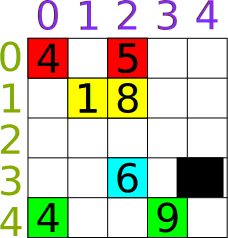
\includegraphics[width=0.25\textwidth]{matrix_format}
        }%
        \subfigure[Stockage COO]{%
           \label{fig:COO}
           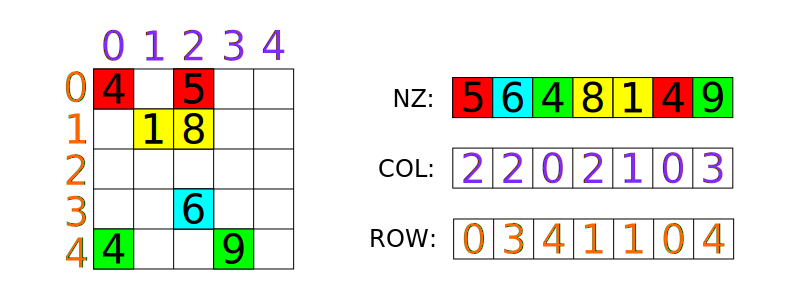
\includegraphics[width=0.35\textwidth]{COO}
        }%
        \subfigure[Stockage CSR]{%
            \label{fig:CSR}
            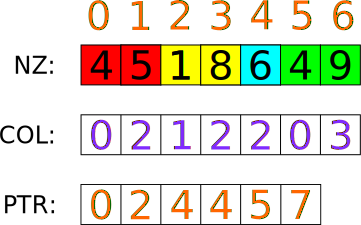
\includegraphics[width=0.35\textwidth]{CSR}
        }%
    \end{center}
    \caption{Comparaison entre les formats de stockage de matrices creuses COO and CSR.}
    \label{fig:matrix_storage}
\end{figure}

Le choix du format de stockage va avoir beaucoup d'effet sur les performances d'une application.
%
Avec la plupart des formats, nous aurons au moins deux accès mémoire pour obtenir les coordonnées 2D d'un coefficient non nul alors qu'avec l'algèbre linéaire dense nous pouvons calculer ces coordonnées à partir de la position dans la matrice.
%
Une partie non négligeable de la bande passante mémoire est utilisée juste pour les coordonnées 2D.
%
Les propriétés creuse et irrégulière de ces matrices impliquent aussi une mauvaise efficacité mémoire des noyaux d'algèbre linéaire creux à cause d'une mauvaise réutilisation du cache.
%
La plupart des optimisations faites en algèbre linéaire dense ne peuvent pas être appliquées à l'algèbre linéaire creuse à cause de l'irrégularité dans l'ordre des calculs ainsi que dans les accès mémoire.
%
Mais l'algèbre linéaire creuse nous permet de résoudre des problèmes bien plus grands que ceux qui utilisent l'algèbre linéaire dense.
%
Ceci est dû au fait qu'avec une taille de matrice équivalente, l'algèbre linéaire creuse utilise vraiment moins de mémoire que l'algèbre linéaire dense.


Résoudre des problèmes linéaires creux est aussi très différent de résoudre des problèmes denses.
%
Nous ne pouvons pas utiliser une inversion directe de matrice, ou la technique de l'élimination de Gauss parce que nous obtiendrions une matrice quasi-dense.
%
Or une matrice quasi-dense avec de grandes dimensions ne pourrait pas tenir en mémoire et même si c'était le cas, le nombre de calculs serait trop important.
%
Donc des méthodes différentes ont été inventées pour être capable de résoudre ces problèmes, beaucoup sont basées sur des méthodes itératives.
%
Nous démarrons donc avec une solution, ensuite ces méthodes réduisent itérativement la différence entre notre solution approximée et la solution réelle.
%
\`{A} la fin, nous obtenons une bonne approximation de la solution, ce qui est souvent suffisant pour être considérée comme la solution au problème.

%+++++++++++++++++++++++++++++++


%+++++++++++++++++++++++++++++++
\section{Résoudre de grands systèmes linéaires creux}
%-------------------------------
\subsection{Preconditioned GMRES}
GMRES\footnote{Generalized Minimal RESidual} method is an iterative method used to solve system of linear equation.
%
This method can be used with any matrix since the matrix is invertible.
%
The GMRES algorithm is composed of some vectors operations and a SpMV\footnote{sparse matrix-vector product}.

As matrices used in reservoir simulation are not well conditioned, the GMRES algorithm converge after a lot of iterations.
%
In this case, we need to precondition the matrix to make the GMRES converges faster.
%
A good preconditioner for our matrices is ILU\footnote{Incomplete LU factorization}.
%
LU factorization consists of factorizing a matrix $A$ into two triangular matrices $L$ and $U$.
%
Then to solve $Ax=b$ is the same as solving $Ly=b$ and $U.x=y$, which can be do easily because $L$ and $U$ are triangular matrices.
%
In case of sparse linear problems, the sparse matrix $A$ become too dense, a lot of zero values become non-zero values and the size to store the matrix in memory become too high.
%
To maintain a reasonable among of memory usage, one can only do some part of the factorization, this is called incomplete LU factorization.
%
With ILU we will try to obtain a sparse pattern for $L$ and $U$ as close as possible the sparse pattern of $A$.

There are two ways to apply ILU in GMRES :
\begin{itemize}
  \item Left preconditioning : $A^{-1}(Ax)=b$
  \item Right preconditioning : $A(A^{-1}x)=b$
\end{itemize}

In programming term, this means that the SpMV must be done before or after the TRSV.

%-------------------------------
\subsection{Domain decomposition}
Domain decomposition is a method to solve large problem by splitting them into smaller problems.
%
This method allow us to parallelize the GMRES when we use a distributed memory paradigm like MPI.
%
Each MPI process manages a subset of cells in the reservoir simulation and is able to do MPI communication on border of the domain.
%
However, the ILU preconditioner is sensible to the number of domain, the GMRES convergence is degraded when the number of domain is too high.

%-------------------------------
\subsection{Cas d'étude}
Pour être en mesure de tester notre méthode de parallélisation en mémoire partagée, nous utilisons un code de solveur linéaire développé à Total SA.
%
Nous allons essayer de paralléliser la partie GMRES préconditionné du code.
%
Dans le but d'évaluer le gain de performance, nous avons choisi des systèmes linéaires à résoudre avec le solveur linéaire.

Ces systèmes linéaires sont représentés sous la forme d'une matrice et d'un vecteur second membre.
%
La structure des matrices est dépendante du problème simulé.
%
Nous utilisons un maillage structuré avec un schéma de discrétisation en 7 points (e.g., volume fini).
%
En gardant une numérotation naturelle, nos matrices aurons donc une structure composée de sept diagonales.
%
En fonction de ce que nous voulons simuler, les entrées de la matrice pourront être scalaires ou composé de petits blocs.
%
Si nous ne simulons que la pression, nous aurons des entrées scalaires.
%
Les simulations de type {\em black-oil} sont les plus utilisées en simulation de réservoir.
%
Il s'agit de simuler 3 variables primaires, la concentration en huile, en gaz et en eau de chaque cellule.
%
Il arrive aussi que l'on souhaite simuler plus précisément les différents types d'huiles contenues dans les réservoirs.
%
Dans ce cas, nous utiliserons un modèle compositionnel dans lequel chaque variable primaire correspondra à la saturation d'un type d'hydrocarbure.
%
Pour les cas black-oil et les cas compositionnels, les entrées de la matrice seront de petits blocs denses de taille $npri*npri$ où $npri$ est les nombres de variables primaires.

Pour évaluer notre code, nous allons utiliser le cas test SPE10 qui est basé sur les données prises du second modèle du 10ème cas test SPE\cite{SPE10}.
%
C'est un réservoir de 1~122~000 de cellules, organisées dans une grille 3D cartésienne de taille 60~x~220~x~85.
%
Il s'agit d'un modèle black-oil, donc à 3 variables primaires, et c'est un problème de référence dans l'industrie pétrolière.
%
Les autres cas tests seront générés par un programme développé en interne, nous utiliserons un cas pression, un cas black-oil et un cas compositionnel à 8 composants.
%
Ce programme génère des cubes 3D cartésiens de taille arbitraire.
%
Ces cas générés nous permettent de tester différentes combinaisons de tailles dans le but d'évaluer le passage à l'échelle de nos algorithmes.

La partie GMRES du code que nous souhaitons paralléliser est composée de plusieurs noyaux d'algèbre linéaire creux.
%
Il y a la factorisation ILU et les résolutions triangulaires, le produit matrice vecteur creux et le produit scalaire.
%
Le parallélisme exploitable dans ces noyaux est différent, il peut être plus ou moins difficile à exploiter.
%
Dans le cas du produit matrice vecteur creux, la multiplication de chaque ligne de la matrice est indépendante, le parallélisme s'exploite facilement.
%
De même pour le produit scalaire, chaque élément du vecteur peut être traité indépendamment.
%
Pour la factorisation ILU c'est différent, certaines lignes doivent être factorisées avant d'autres, le parallélisme est donc plus dur à exploiter.
%
Les résolutions triangulaires se parallélisent de la même façon que la factorisation ILU.
%
Dans la suite de la thèse, nous expliquerons comment exploiter efficacement le parallélisme dans ces quatre cas.

%+++++++++++++++++++++++++++++++


%+++++++++++++++++++++++++++++++
\section{\'Evolution des architecture}
%-------------------------------
\subsection{Processeurs mono-coeur}
Pour être capable de simuler de grands problèmes physiques, nous avons besoin de beaucoup de puissance de calcul.
%
Cette puissance se mesure en FLOPS\footnote{FLoating-point Operations Per Second}, il s'agit du nombre d'opérations par seconde qu'un ordinateur peut effectuer sur des nombres à virgules flottantes.
%
Même les processeurs mono-coeur peuvent faire des opérations en parallèle.
%
Le parallélisme au niveau instruction en est un bon exemple, les pipelines d'instructions permettent de paralléliser les différentes étapes liées au traitement d'une exécution.
%
Dans l'idéal, le processeur utilisant un pipeline d'instruction pourra exécuter une opération par cycle, donc un processeur à 4~GHz aura une puissance de calcul de 4~GFLOPS si les opérations flottantes sont faites en 1 cycle.


Par la suite, les processeurs ont gagnés des instructions permettant d'effectuer une même opération sur des données différentes, aussi appelées instructions SIMD dans la taxonomie de Flynn.
%
Ces processeurs dits vectoriel peuvent donc avoir une puissance de calcul supérieur, si une instruction est capable d'effectuer 4 opérations à la fois et qu'il tourne à 4~GHz, alors il aura une puissance de calcul de 16~GFLOPS.
%
Il s'agit ici d'une puissance théorique, tous les codes de calculs n'ont pas la possibilité d'exploiter les instructions vectorielles.
%
Ces instructions sont souvent utilisées dans les noyaux de calculs d'algèbre linéaire dense.
%
En simulation de réservoir, nous utilisons ces noyaux de calculs sur les blocs de nos matrices.

%-------------------------------
\subsection{Processeurs multi-coeur}
Pour obtenir encore plus de parallélisme, il est possible de multiplier les unités de calcul au sein d'un processeur.
%
Ces unités de calcul, aussi appelées coeurs de calcul, peuvent être considérées comme des processeurs.
%
Chaque coeur a son propre pipeline d'instructions, ses registres et ses unités arithmétiques.
%
Les coeurs partagent un ou plusieurs niveaux de cache entre eux ainsi que le bus d'accès à la mémoire.
%
La puissance de calcul d'un processeur à 4 coeurs composés d'unités vectoriels et chaque coeur tournant à 4~GHz est de 64~GFLOPS.

%-------------------------------
\subsection{SMP}
Pour encore gagner de la puissance, nous pouvons connecter plusieurs processeurs ensemble.
%
Ces processeurs se partagent les ressources disponibles sur la carte mère, cela inclut les entrées/sorties et la mémoire.
%
La façon d'inter-connecter tous les processeurs avec la carte mère peut différer entre différentes architectures.
%
Avec l'architecture SMP, tous les processeurs sont connectés à un bus de données et un arbitre choisit quel processeur peut utiliser le bus à un instant donné (Fig.~\ref{fig:smp}).
%
Cette conception ne passe pas à l'échelle au niveau des performances quand le nombre de processeurs grandit.
%
La bande passante est partagée par tous les processeurs et l'arbitre du bus devient un goulot d'étranglement.
%
Pire, la latence d'un accès mémoire va dépendre de la congestion du bus mémoire.
%
L'utilisation de 4 processeurs comme décrit précédemment donne une puissance de calcul de 256~GLOPS.
%
Cette puissance de calcul ne prend pas en compte les limitations mémoires.
%
Pour pouvoir atteindre cette puissance, il faut limiter les accès à la mémoire partagée et privilégier les accès à la mémoire cache.

%   (-_-)   %
\begin{figure}[!h]
        \centering
        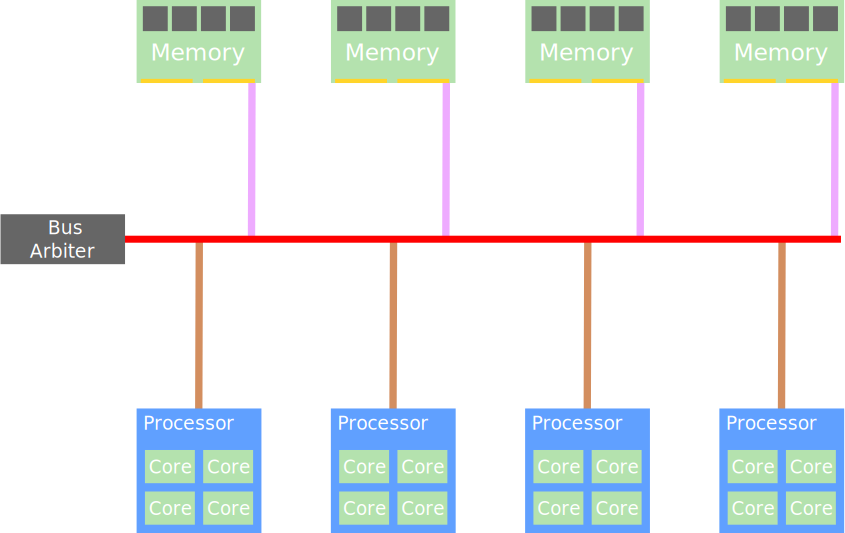
\includegraphics[width=0.8\textwidth]{smp}
        \caption{Vue d'ensemble d'une architecture à accès mémoire uniforme (SMP).}
        \label{fig:smp}
\end{figure}

%-------------------------------
\subsection{NUMA}
To override the limitations of SMP architecture, the memory can be physically distributed over processors (Fig.~\ref{fig:numa}).
%
With NUMA architecture, latency and bandwidth of each memory access depend on the distance between the processor and the physical locality of the memory.
%
There are several ways to interconnect processors, by connecting all processors together all-to-all the latency can be the lowest possible but once again it's not scalable.
%
It's also possible to connect only some processors together and try to optimize the number of hops like it is done in cluster.
%
At the end, the distance between each NUMA bank can be represented under a matrix form.

%   (-_-)   %
\begin{figure}[!ht]
  \centering
  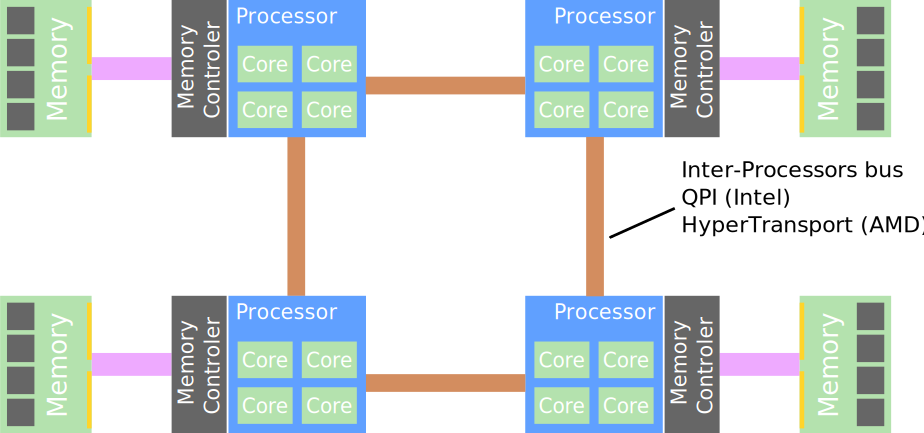
\includegraphics[width=0.8\textwidth]{numa}
  \caption{Overview of an NUMA architecture}
  \label{fig:numa}
\end{figure}

%-------------------------------
\subsection{Grappe de serveurs}
Au final, il est possible de connecter plusieurs ordinateurs entre eux pour obtenir une machine encore plus puissante.
%
Chaque ordinateur est appelé noeud de calcul, il a sa propre mémoire, fait tourner son propre système d'exploitation et peut être considéré comme une machine isolée.
%
Les noeuds sont reliés entre eux par un réseau à faible latence/haut débit, tel que Infiniband ou Myrinet.
%
Le principal avantage de cette solution est le passage à l'échelle.
%
Il est possible de construire des machines de très grandes tailles et très puissantes.



Parmi les 500 machines les plus puissantes au monde au moment de l'écriture de cette thèse, 429 sont des grappes de serveurs.
%
La machine la plus puissante est la {\em TIANHE-2} avec une puissance crête d'environ 55~PFLOPS.
%
Mais l'utilisation de ces machines pose un sérieux problème, elles ne sont pas vraiment faciles à programmer.
%
Il faut prendre en compte que la mémoire n'est pas globale, chaque noeud ne voit que sa mémoire locale.

%-------------------------------
%\subsection{Many-core}
Another solution, used by Intel in the Xeon Phi coprocessor, is to use a ring bus (See Fig~\ref{fig:interconnect}).
%
Memory is distributed over the ring bus just as core units.
%
Why is it better than an SMP ?
%
During my thesis, I had the opportunity of trying a Xeon Phi.


%   (-_-)   %
\begin{figure}[!ht]
  \centering
  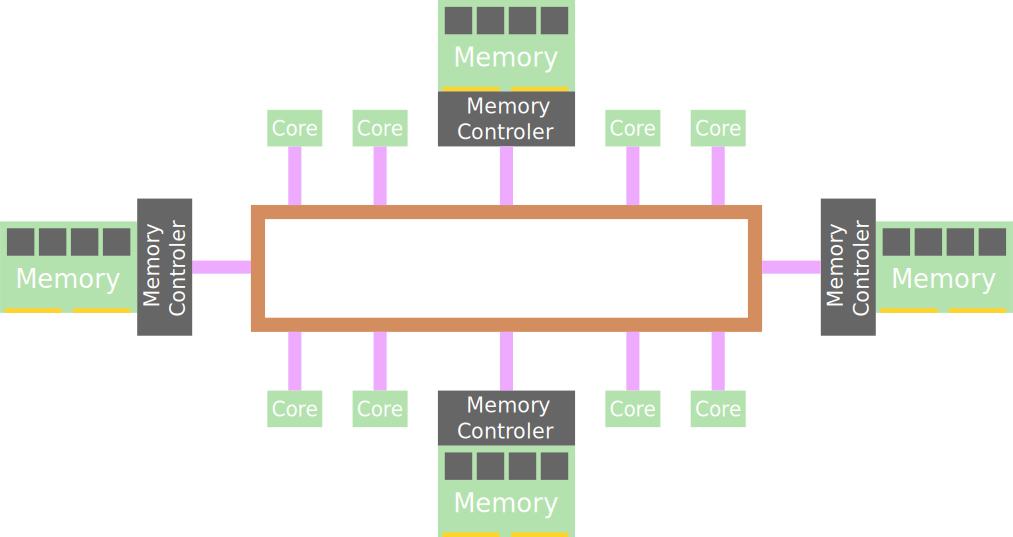
\includegraphics[width=0.8\textwidth]{interconnect}
  \caption{Overview of Xeon Phi Architecture}
  \label{fig:interconnect}
\end{figure}

  \begin{itemize}
    \item Xeon phi
    \item GPU ?
    \item Too many change in program but not always performance (data transfer)
  \end{itemize}

%-------------------------------
\subsection{Nos machines}
Dans le but d'étudier différents problèmes liés à la programmation par tâche, nous avons sélectionné deux machines avec des architectures différentes.

\subsubsection{Rostand}
Rostand est une grappe de serveurs appartenant à Total S.A. company.
%
Elle est composée de 640 noeuds de calcul interconnectés avec un réseau Infiniband.
%
Chaque noeud est lui-même composé de 2 banc NUMA avec un processeur Intel Xeon X5660 et 24~GO de mémoire par banc NUMA (Fig.~\ref{fig:rostand}).
%
Les processeurs ont 6 coeurs, soit un total de 12 coeurs par noeud de calcul et 7680 coeurs pour l'ensemble de la grappe.

%   (-_-)   %
\begin{figure}[!ht]
        \centering
        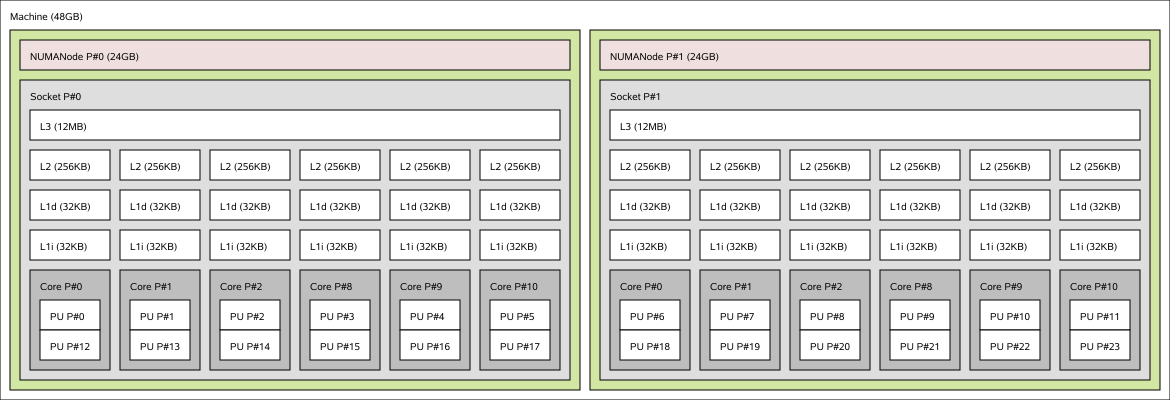
\includegraphics[width=\textwidth]{rostand_lstopo}
        \caption{Topologie d'un noeud de calcul de Rostand. Le schéma a été obtenu avec le logiciel hwloc.}
        \label{fig:rostand}
\end{figure}

Avec cette machine, nous allons pouvoir tester deux paradigmes de programmation parallèle.
%
Dans un premier temps nous allons faire du parallélisme intra-noeud puis nous verrons le parallélisme inter-noeud.

\subsubsection{Manumanu}
Manumanu est une machine Altix UV100, cet ordinateur est composé de 20 bancs NUMA.
%
Chaque banc NUMA est composé d'un processeur Intel Xeon E7-8837 ainsi que de 32~GO de mémoire.
%
Les processeurs ont chacun 8 coeurs de calcul, pour un total de 160 coeurs et 640~GO de mémoire partagée.
%
Cette machine est vraiment intéressante pour évaluer les effets NUMA.

%   (-_-)   %
\begin{figure}[!ht]
     \begin{center}
        \subfigure[Matrice des distances entre chaque banc NUMA. Résultat obtenu avec la commande ``numactl --hardware''.]{%
          \label{fig:manumanu_distance}
          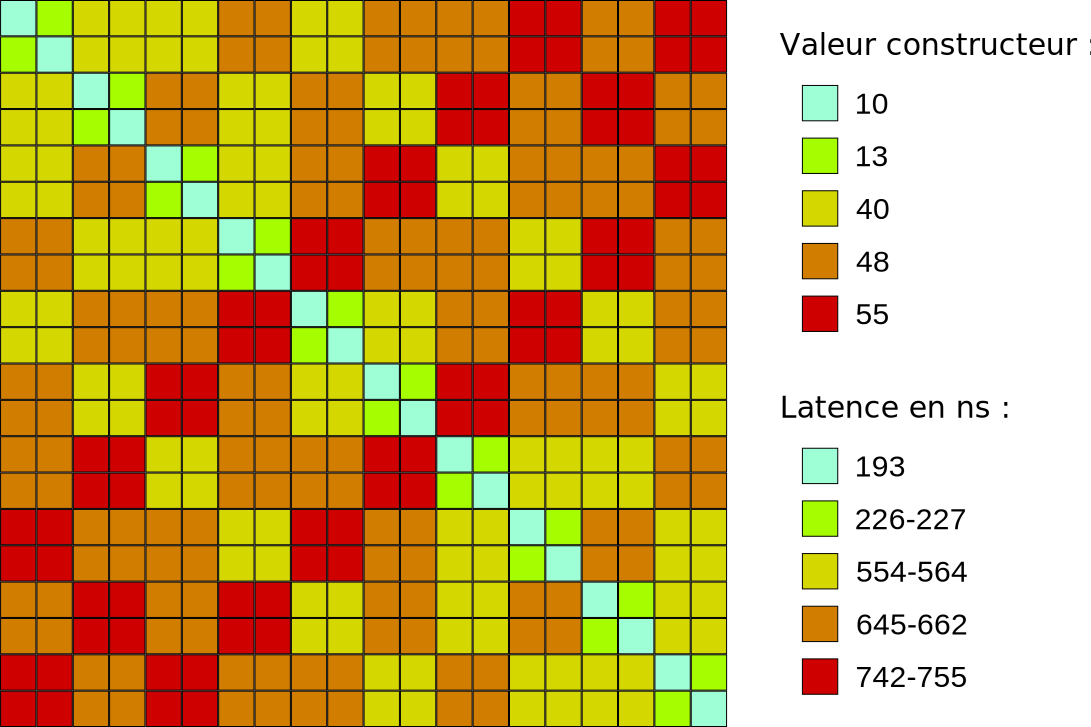
\includegraphics[width=0.49\textwidth]{manumanu_distance}
        }%
        \subfigure[Topologie de Manumanu déduite de la matrice des distances. Chaque noeud représente un ensemble de deux bancs NUMA.]{%
          \label{fig:manumanu_topo}
          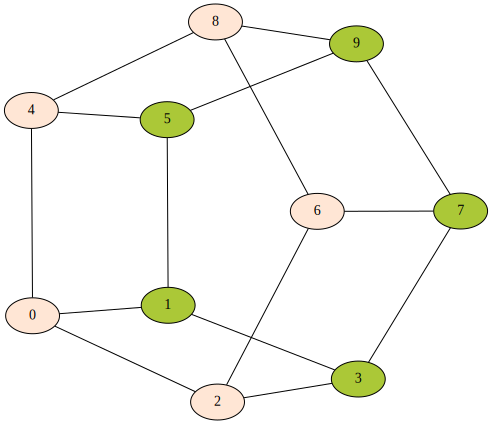
\includegraphics[width=0.49\textwidth]{manumanu_topologie}
        }%
    \end{center}
    \caption{Architecture de Manumanu.}
    \label{fig:manumanu}
\end{figure}

\`{A} partir de la matrice des distances (Fig.~\ref{fig:manumanu_distances}), nous pouvons déduire la topologie de la machine.
%
Les bancs NUMA sont regroupés deux par deux et chaque groupe est connecté à trois autres groupes.
%
Ce regroupement permet de limiter la distance maximal entre deux banc NUMA, il y aura au maximum 3 sauts.

%+++++++++++++++++++++++++++++++


%+++++++++++++++++++++++++++++++
\section{Parallélisme multi-coeur}
%-------------------------------
Lorsque l'on souhaite paralléliser un code de calcul, on se retrouve à devoir choisir parmi plusieurs paradigme de parallélisation.
%
Le choix de ce paradigme est une étape importante, elle déterminera les algorithmes à utiliser et donc aussi les performances du programme.
%
En effet, un même problème ne se résoudra pas de la même façon en fonction du paradigme choisi.
%
Mais le choix du paradigme est aussi déterminé par l'architecture de la machine cible.
%
Dans le cas d'une grappe de serveurs, on préféra un paradigme par passage de messages qui nous obligera à utiliser des algorithmes distribués. %%% TODO ST: Pourquoi est-ce bien?
%
Alors que dans le cas d'une machine à mémoire partagée nous aurons recours à l'utilisation de processus légers, aussi appelé {\em thread}.
%
Plusieurs paradigmes peuvent être utilisés ensemble, nous pouvons ainsi tirer parti des avantages de chacun tout en limitant leurs inconvénients.
%
Nous allons maintenant détailler les différents paradigmes de parallélisation que nous avons utilisé.

%-------------------------------
\subsection{Passage de messages}
Certaines machines ne fonctionnent pas avec une mémoire globale, mais avec une mémoire distribuée.
% 
Chaque noeud de calcul a une mémoire locale et ne peut pas accéder directement à la mémoire des autres noeuds distants.
%
Avec le paradigme de passage de messages, chaque processus a son propre espace mémoire virtuel et communique avec les autres processus par le biais d'envoi/réception de messages.
%
Ces communications se font à l'aide d'une interface de programmation qui fournit des fonctions permettant l'échange de messages point-à-point.
%
L'interface la plus connue et la plus utilisée actuellement est MPI\footnote{Message Passing Interface}.
%
Elle permet de faire communiquer deux processus ensemble sans se soucier du réseau utilisé ni même de la différence d'encodage des entiers ({\em little endian}/{\em big endian}) entre deux architectures différentes.

L'un des avantages majeurs de ce paradigme est qu'il permet d'utiliser un ensemble très varié de machines.
%
Il fonctionne aussi bien en mémoire partagée qu'en mémoire distribuée.
%
Son utilisation en mémoire partagée permet de n'utiliser qu'un seul type de parallélisme dans un programme.
%
Un programme pur MPI peut donc utiliser tous les coeurs d'un noeud de calcul avec le même code source qui permet d'utiliser des grappes de serveurs.
%
Mais il ne s'agit pas toujours de l'implémentation la plus efficace pour paralléliser un code, il est souvent plus performant d'utiliser une parallélisation hybride MPI+Threads\cite{mpi_openmp}.
%
De plus, certains algorithmes ne peuvent pas être écrits efficacement avec ce paradigme.
%
Par exemple, dans notre cas la factorisation d'une matrice creuse se parallélise très mal en mémoire distribuée.
%
Nous ne pouvons extraire du parallélisme qu'entre les factorisations de ligne de la matrice.
%
Or ce niveau de granularité du calcul ne donne pas de bonnes performances avec un paradigme par passage de messages.
%
Nous sommes donc obligés de modifier les méthodes de factorisation pour être capables d'obtenir de la performance.
%
La méthode de Jacobi par blocs permet d'effectuer en parallèle une factorisation sur chaque bloc au détriment de la convergence de la méthode itérative.
%
C'est donc cette méthode qui est utilisée pour une parallélisation par passage de messages.
%
Cette méthode a l'inconvénient d'ignorer de nombreuses connexions entre les cellules du réservoir et fournit donc un préconditionnement de moins bonne qualité qu'une factorisation ILU sur la matrice complète.

%-------------------------------
\subsection{Parallel for loop}
One of simplest way to obtain a multi-threaded program is to share the work done in a computational time consuming loop across all physical cores available.
%
This method has been democratize by OpenMP and its famous ``\#pragma omp parallel for'' which is a C compiler directive that do the work for us.
%
To be able to use this directive, all iterations of the loop must be independent, in other terms, if we have an infinite number of processor we are able to do all iterations at the same time.
%
Performance of this type of parallelization are often quite enough for a lot of software, but sometimes the parallelism can't be express under a parallel loop because of dependencies between data.
%
In this case, another type of parallelism must be use.


%% TODO
%% Expliquer que les pragmas se désactivent facilement, il s'agit de parallelism quasi automatique
%%

%-------------------------------
\subsection{Task paradigm}
Task paradigm can used to describe a set of computational part with strict order between some part.
%
It is usually represented under a DAG\footnote{Direct Acyclic Graph} form, nodes are computational part and edges are dependencies between nodes.
%
This representation describe naturally the parallelism of a problem.
%
This graph is then used by a task scheduler which will choice to affect a specific task to a core.

%+++++++++++++++++++++++++++++++


%+++++++++++++++++++++++++++++++
\section{Runtime}
%-------------------------------
\subsection{Vue d'ensemble}
Un moteur d'exécution, ou {\em runtime}, est un morceau de logiciel utilisé par d'autres logiciels pour abstraire des parties du système.
%
L'idée principale est {\em compiler une fois, exécuter partout}.
%
Ils sont présent un peu partout et peuvent avoir différentes fonctions.
%
Certains langages dits de haut niveau utilisent un runtime, par exemple Java a un runtime pour gérer son ramasse-miettes.
%
Toutes les implémentations de MPI ont un runtime.
%
Les cadriciels de programmation à base de tâches tendent à utiliser un runtime.
%
Les parties suivantes se concentreront sur le support des runtimes pour la programmation à base de tâches.


Les runtimes utilisés pour la programmation à base de tâches doivent en premier lieu être capable d'ordonnancer le traitement des tâches tout en respectant l'ordre des dépendances entre les tâches (Fig.~\ref{fig:runtime}).
%
Ces runtime doivent aussi fournir un équilibrage de charge entre toutes les ressources matérielles disponibles (potentiellement hétérogènes) dans le but de minimiser le temps de calcul.
%
Certains runtimes s'occupent de transférer des données entre deux ressources potentiellement hétérogènes, comme par exemple entre la mémoire principale et la mémoire d'une carte graphique ou plus simplement entre deux processus.
%
Ces transferts peuvent être implicites, le runtime a connaissance des données qui sont manipulées, ou ils peuvent être explicites avec l'utilisation d'une tâche spéciale qui s'occupera de faire les échanges de données.

%   (-_-)   %
\begin{figure}
  \centering
  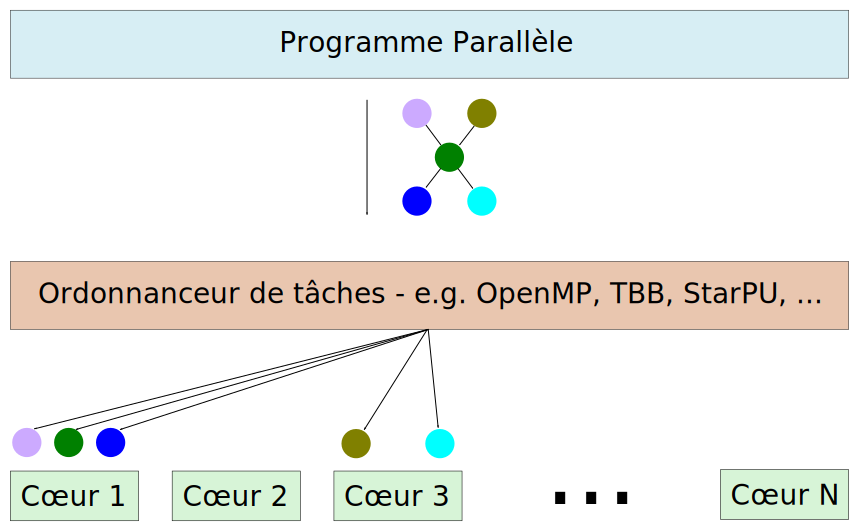
\includegraphics[width=0.8\textwidth]{runtime}
  \caption{Le programme parallèle fournit un graphe de tâches à l'ordonnanceur de tâches. Les tâches sont ensuite distribuées sur les coeurs de calcul disponibles.}
  \label{fig:runtime}
\end{figure}


Pour améliorer l'équilibrage de charge, les runtimes ont des politiques d'ordonnancement, la plupart de ces politiques sont dynamiques et peuvent s'adapter à la charge courante de la machine.
%
D'autres politiques d'ordonnancement, dîtes statiques, permettent de réduire le coût d'ordonnancement.
%
L'ordonnanceur parfait n'existe pas et n'existera sûrement jamais.
%
En effet, trouver le meilleur ordonnancement d'un ensemble de tâches avec un nombre limité de ressources de calcul est un problème NP-complet\footnote{Un problème est NP-complet si le temps nécessaire à la résolution du problèmes est polynomial comparé à la taille des données en entrées et que ce problème soit aussi difficile que tous les autres problèmes NP-complets.}.
%
Il existe des heuristiques d'ordonnancement qui donnent de bons résultats dans la majorité des cas, nous pouvons citer l'algorithme HEFT\cite{heft}.
%
Si le modèle de programmation le permet, des informations additionnelles peuvent être attribuées aux tâches, comme par exemple une estimation du temps de calcul, ces informations sont ensuite utilisées par l'ordonnanceur pour améliorer le placement des tâches.


L'apparition des premières machines parallèles à mémoire partagée a conduit à la recherche de nouvelles méthodes pour les programmer.
%
Il faut donc distribuer une charge de travail sur plusieurs unités de calcul.
%
Malheureusement, il arrive que cette charge de travail de soit pas connu l'avance.
%
Une idée est alors apparu pour rendre cette distribution plus flexible : le vol de travail (ou {\em work-stealing} en anglais).
%
Dès qu'une ressource de calcul n'as plus de travail, elle essaye de voler du travail à une autre ressource.
%
Le langage Cilk~\cite{Cilk}, apparu en 1994 et toujours développé sous le nom Cilk++~\cite{Cilk++}, permet de faire du vol de travail.
%
Les tâches sont décrites par le programmeur avec des mots clés additionnels au langage C, par exemple le mot-clé {\em spawn} placé avant l'appel d'une fonction permet à Cilk de comprendre qu'il doit créer une nouvelle tâche et qu'il doit l'ordonnancer.
%
Ces tâches sont empilées sur une pile spécifique à chaque thread.
%
Le vol de tâche se fait par le biais de cette pile de tâches.


Peu de temps après, en 1997, une interface de programmation parallèle voit le jour, il s'agit d'OpenMP~\cite{OpenMP}.
%
Les premières versions d'OpenMP se concentrent sur le parallélisme de boucle.
%
Ce n'est qu'en 2008 que le support des tâches est ajouté à OpenMP dans sa version 3.0.



Plus récemment, à la fin des années 2000, la révolution du GPGPU donne lieu à l'apparition de nouveaux runtime.
%
Les premières méthodes permettant d'utiliser un GPU pour du calcul étaient rudimentaires.
%
Il s'agissait de détourner l'utilisation des shaders programmables des interfaces de programmation graphiques comme par exemple OpenGL.
%
Puis des langages spécifiques on vus le jour, parmi ceux ci, le plus populaire sont CUDA et OpenCL.
%
CUDA est développé par NVidia et ne permet de programmer que des GPU NVidia.
%
OpenCL est une spécification du Khronos Group est a pour but de fournir une interface de programmation standard pour programmer toutes sortes d'accélérateurs.
%
Ces accélérateurs peuvent être des GPUs mais de manière générale il s'agit de co-processeur déporté.




StarPU~\cite{starpu}, développé à Inria permet de d'écrire plusieurs versions d'une routine à la fois pour le CPU et le GPU.
%
Ces morceaux de codes spécifiques à une architecture sont appelés {\em codelet}.
%
Puis les stratégies d'ordonnancement intégrées à StarPU choisiront la codelet qui permettra d'obtenir le meilleur temps de calcul.
%
Ce choix prend aussi en compte le temps de transfert mémoire entre la mémoire centrale et la mémoire du GPU.
%
Pour avoir une gestion efficace de ces transferts mémoires, StarPU implémente un gestionnaire mémoire.
%
Ce gestionnaire est capable d'effectuer des transferts entre toutes les zones mémoires de la machine (mémoire centrale, mémoire GPU, disques, ...) et de maintenir la cohérence des données.
%
Par exemple, si une donnée A est en mémoire centrale et qu'une codelet doit l'utiliser sur le GPU, il y aura d'abord une copie A vers la mémoire du GPU.
%
Ensuite tant que cette donnée n'est accédée qu'en lecture, il y aura deux copies valides, une en mémoire centrale et une en mémoire GPU.
%
Dès qu'une codelet accède à la donnée en écriture, toutes les autres copies sont invalidées et un transfert mémoire sera nécessaire pour les mettre à jour.
%
StarPU intègre aussi plusieurs politiques d'ordonnancement
%
L'équipe de développement met aussi en avant la possibilité d'écrire son propre ordonnanceur et de l'intégrer à StarPU.




OmpSs~\cite{OMPSs} est un runtime qui permet tout comme StarPU d'écrire du code à la fois pour le CPU et pour le GPU puis de laisser le runtime choisir parmi toutes les versions d'une fonction.
%
La différence entre ces deux runtimes provient surtout de la description du parallélisme.
%
OmpSs propose un approche à base d'annotation de code en étendant la spécification OpenMP version 3.
%
Cette extension permet au mot clé {\em task} d'être accompagné d'informations complémentaires sur l'utilisation des paramètres en entrée.
%
Le programmeur doit toujours écrire le code spécifique à chaque architecture précédé d'informations concernant la fonction implémentée ainsi que l'architecture cible.




PaRSEC~\cite{PaRSEC} est un runtime développé à l'ICL permettant de travailler directement en mémoire distribuée.
%
Le parallélisme dans PaRSEC doit être décrit dans un langage spécifique, le JDF.
%
L'ensemble des tâches du programme est décrit dans ce langage et ce n'est que la distribution des données en mémoire distribuée qui détermineras le processus qui exécuteras la tâche.
%
PaRSEC s'occupe automatiquement des communications entre processus permettant de maintenir une cohérence entre les données.
%
L'inconvenient majeur de ce runtime est son manque de flexibilité.
%
Le format JDF ne permet de créer dynamiquement de nouvelle tâche.



HMPP~\cite{hmpp} est un runtime adressant le problème de la programmation hybride CPU/GPU.
%
Il s'utilise avec des annotations de code à la manière d'OpenMP.
%
Puis le code annoté est ensuite transformé par un compilateur source-to-source vers un autre langage spécifique à l'architecture cible, comme le CUDA par exemple.
%
Les transferts mémoires entre la mémoire centrale et la mémoire du GPU sont soit implicite au moment de l'appel de la codelet mais cette méthode ne permet de recouvrir la communication par du calcul.
%
Soit explicite avec l'ajout d'annotation, il est donc à la charge du programmeur de choisir le bon moment pour transférer les données.



OpenACC~\cite{OpenACC} est un standard de programmation développé par un consortium de société dans le but de simplifier la programmation parallèle hybride CPU/GPU.
%
Les spécificités de ce standard ressemble en de nombreux points à HMPP (annotations, gestion mémoire, ...).
%
Son principal avantage est qu'il est soutenu par plusieurs sociétés là où HMPP n'a plus personne.
%
OpenMP ajoute dans version 4 le support de la programmation hybride, son fonctionnement est identique à OpenACC, seuls les mot-clés changent.





Parmi ces runtimes on trouve X-KAAPI~\cite{xkaapi}.

%+++++++++++++++++++++++++++++++




%=========================================================
\chapter{Un problème de granularité}
\minitoc
\vspace{1cm}
%=========================================================
%+++++++++++++++++++++++++++++++
\section{Parallélisation de l'algorithme GMRES préconditionné}
%-------------------------------
\subsection{Partie GMRES}
L'algorithme GMRES est utilisé pour résoudre de grands systèmes linéaires creux.
%
La plupart des opérations sont des opérations de type BLAS1 (axpy, dot product...) et sont facilement parallélisables\cite{para_blas}.
%
L'opération la plus coûteuse de l'algorithme du GMRES non préconditionné est le produit matrice vecteur, ou {\em SpMV}\footnote{Sparse Matrix Vector multiply}.
%
Chaque ligne de la matrice peut être traitée indépendamment les unes des autres.
%
Parmi les choix de parallélisation que nous avons à notre disposition, nous allons choisir du parallélisme de boucle\cite{para_spmv}.
%
En effet, il permet d'utiliser une granularité adaptative contrairement au parallélisme à base de tâches qui impose le choix d'une granularité.
%
Il permet aussi d'avoir un bon équilibrage de charge avec possibilité de vol de travail là où un paradigme par passage de messages impose un découpage fixe de la charge de travail.



Donc de manière générale, l'algorithme du GMRES se parallélise très bien.
%
Mais nous ne pouvons pas l'utiliser tel quel, nos matrices ne sont pas assez bien conditionnées.
%
Il est nécessaire d'utiliser un préconditionneur pour nos matrices afin obtenir de bonnes performances.
%
Par contre, la partie préconditionneur n'est pas toujours facilement parallélisable.
%
Par exemple, le préconditionneur ILU(k), que nous allons utiliser, est un algorithme dont le parallélisme dépend de la structure de la matrice.
%
Cette structure dépend elle-même du problème traité ainsi que de la numérotation des cellules (Fig.~\ref{fig:matrix_ordering}).
%
Dans le cas d'une numérotation naturelle, le parallélisme est difficile à exploiter.
%
Nous sommes obligés d'utiliser du parallélisme à base de tâches, potentiellement moins performant que du parallélisme de boucle.
%
En changeant la numérotation des cellules, nous pouvons changer le graphe de tâches.
%
Par exemple, lorsque nous factorisons une matrice nous devons procéder ligne par ligne.
%
Les dépendances de factorisation entre les lignes de la matrice ne vont donc que dans un sens, de la plus petite vers la plus grande.
%
Une numérotation rouge-noire consiste à colorier le graphe représentant notre réservoir de façon à n'avoir aucune connexion entre deux cellules d'une même couleur.
%
Dans le cas d'un maillage 2D structuré, nous pouvons colorier facilement le graphe en parcourant les cellules une à une.
%
La numérotation se fait ensuite en numérotant successivement toutes les cellules d'une même couleur puis en numérotant toutes les cellules de l'autre couleur avec des nombres strictement supérieurs à ceux de la première couleur.
%
Par exemple sur la figure~\ref{fig:matrix_redblack_reservoir}, les cellules 1 à 8 sont rouges et les cellules 9 à 16 sont noires.
%
Les dépendances iront toujours des cellules rouges vers les cellules noires.
%
Nous pouvons donc dans un premier temps factoriser toutes les lignes de la matrices qui correspondent aux cellules rouges.
%
Puis dans un second temps, nous pouvons factoriser les autres lignes, celles qui correspondent aux cellules noires.
%
Nous avons donc un parallélisme de boucle, souvent plus efficace qu'un parallélisme à base de graphe de tâches.
%
Mais qui dans ce cas-là fournit un moins bon préconditionnement\cite{red_black_ilu2}.
%
Dans le but de garder un bon préconditionnement, ce chapitre sera consacré à exploiter un maximum de parallélisme de l'algorithme ILU(k) tout en gardant une numérotation naturelle.

%   (-_-)   %
\begin{figure}[!h]
     \begin{center}
        \subfigure[Numérotation naturelle des cellules.]{
          \label{fig:matrix_natural_reservoir}
          
\includegraphics[width=0.45\textwidth]{matrix_natural_reservoir}
        }
        ~
        \subfigure[Matrice associé à une numérotation naturelle.]{
          \label{fig:matrix_natural_ordering}
          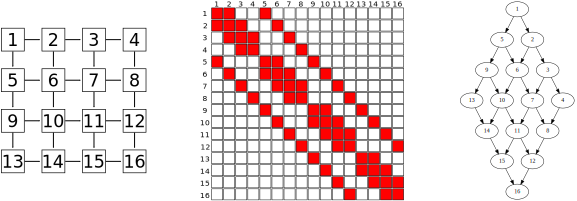
\includegraphics[width=0.45\textwidth]{matrix_natural_ordering}
        }

        \subfigure[Numérotation rouge-noir des cellules.]{
          \label{fig:matrix_redblack_reservoir}
          
\includegraphics[width=0.45\textwidth]{matrix_redblack_reservoir}
        }
        ~
        \subfigure[Matrice associé à une numérotation rouge-noir.]{
          \label{fig:matrix_redblack_ordering}
          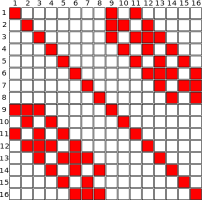
\includegraphics[width=0.45\textwidth]{matrix_redblack_ordering}
        }
    \end{center}
    \caption{Impact de la numérotation sur la structure des matrices creuses.}
    \label{fig:matrix_ordering}
\end{figure}



%% \begin{algorithm}
%%   \fontsize{8pt}{9pt}\selectfont
%%     \begin{algorithmic}[1]
%%       \STATE Compute $r_0 := b - Ax_0$, $\beta := ||r_0||_2$, and $v_1 := r_0/\beta$
%%       \STATE Define the $(m + 1) x m$ matrix $\overset{-}{H}_m = \{h_{ij}\}_{1 \leq i \leq m+1, 1 \leq j \leq m}$. Set $\overset{-}{H}_m = 0$
%%       \FOR{$j=1$ to $m$}
%%         \STATE \tikz[baseline]{\node[fill=yellow!20,anchor=base]{Compute $temp := Triangular\_Solve(M, v_j)$};} \hspace{0.3in} (MPI\_Send(Border\_Cells))
%%         \STATE \tikz[baseline]{\node[fill=red!20,anchor=base]{Compute $w_j := A * temp$};} \hspace{1.2in} (MPI\_Recv(Ghost\_Cells))
%%         \FOR{\tikz[baseline]{\node[fill=blue!20,anchor=base]{$i=1$ to $j$};}}
%%           \STATE \tikz[baseline]{\node[fill=blue!20,anchor=base]{$h_{ij} := (w_j, v_i)$};}
%%           \STATE \tikz[baseline]{\node[fill=blue!20,anchor=base]{$w_j := w_j - h_{ij}v_i$};}
%%         \ENDFOR
%%         \STATE $h_{j+1,j} := ||w_j||_2$.
%%         \IF{$h_{j+1,j} = 0$}
%%           \STATE $m := j$
%%           \STATE \textbf{break}
%%         \ENDIF
%%         \STATE $v_{j+1} := w_j/h_{j+1,j}$
%%       \ENDFOR
%%       \STATE Compute $y_m$ the minimizer of $||\beta{}e_1 - \overset{-}{H}_my||_2$ and $x_m := x_0 + V_my_m$
%%     \end{algorithmic}
%%     \caption{GMRES with Householder orthogonalization from Yousef Saad}
%%   \end{algorithm}

%-------------------------------
\subsection{Partie préconditionneur}
La factorisation LU en algèbre linéaire dense est une méthode pour factoriser une matrice $A$ en deux matrices $L$ et $U$.
%
$L$ est une matrice triangulaire inférieure, toutes les valeurs au-dessus de la diagonale sont nulles.
%
Symétriquement, $U$ est une matrice triangulaire supérieure, toutes les valeurs de $U$ en-dessous de la diagonale sont nulles.
%
Le principal intérêt de cette factorisation est de trouver facilement $x$ dans les équations du type $Ax=y$.
%
Dans le cas où $A=L.U$, le système d'équations $Ax=y$ est transformée en deux systèmes d'équations $L.x_{tmp}=y$ et $U.x=x_{tmp}$.
%
La méthode utilisée pour résoudre les systèmes composés de matrices triangulaires est triviale.
%
Il suffit de résoudre chaque équation ligne par ligne en commençant par la ligne qui n'a qu'une seule valeur non nulle.
%
Ensuite il faut résoudre la ligne avec deux valeurs non nulles dont une des inconnues provient de la solution précédente, et ainsi de suite jusqu'à la dernière ligne.
%
Il existe du parallélisme à exploiter dans cet algorithme, à chaque fois qu'une inconnue est trouvée, on peut la retirer de chacune des lignes restantes à traiter~\cite{plasma_lu}.



En algèbre linéaire creuse, la transformation des éléments nuls de la matrice creuse en éléments non nuls est appelée remplissage.
%
La factorisation LU d'une matrice $A$ creuse donnera deux matrices triangulaires denses $L$ et $U$.
%
Or, si l'on souhaite effectuer la factorisation exacte dans le cas d'une matrice d'ordre élevé ($>$ 100 000), ces deux matrices ne peuvent pas tenir en mémoire.
%
C'est pourquoi en algèbre linéaire creuse, on utilise une version altérée de cette factorisation que l'on appelle factorisation incomplète, ou {\em ILU}\footnote{Incomplete LU}, dont le but est de limiter le remplissage de la matrice.
%
L'algorithme ILU est similaire à l'algorithme LU mais le remplissage est limité par des conditions définies par l'algorithme.
%
Ces conditions peuvent être de deux formes : soit en limitant le remplissage avec une valeur seuil (ILUT\cite{saad1994ilut}), soit en limitant le niveau d'interaction entre les lignes de la matrices (ILU(k)).
%
Dans le cas ILU(k), le paramètre k sert à limiter le niveau d'interaction entre les lignes.
%
Avec $k=0$, le motif des matrices $L$ et $U$ reste similaire au motif de la matrice $A$ (Algo~\ref{algo:ilu0}).


Le parallélisme exploitable dans l'algorithme ILU est différent de celui exploitable dans l'algorithme LU, il offre la possibilité de factoriser certaines lignes en parallèle et ce parallélisme se représente naturellement sous la forme d'un graphe de tâches (Fig.~\ref{fig:example_3_dag}).
%
Chaque tâche représente la factorisation d'une ligne de la matrice et les dépendances entre les tâches sont données par le motif de la matrice.
%
En effet, pour factoriser la ligne $i$, nous devons factoriser toutes les lignes $j$ inférieures à $i$ tel que l'entrée $(i,j)$ de la matrice soit non nulle.
%
Cette dépendance de donnée provient de la ligne~\ref{algo:ilu0:dep} de l'algorithme~\ref{algo:ilu0}.
%
Donc, à partir du motif des valeurs non-nulles de la matrice, nous pouvons facilement construire le graphe de tâche:
%
la tâche $i$ corresponds à la ligne $i$ de la matrice (ligne \ref{algo:ilu0:task_begin} à \ref{algo:ilu0:task_end} de l'algorithme~\ref{algo:ilu0}), la liste des tâches prédécesseurs de la tâche $i$ est donnée par l'index de colonne des valeurs non-nulles avant la diagonale dans la ligne $i$ (ligne~\ref{algo:ilu0:dep}) et la liste des tâches successeurs de la tâche $i$ est donnée par l'index de ligne des valeurs non-nulles au-dessous de la diagonale de la colonne $i$ (Fig.~\ref{fig:example_2_matrix}).

\begin{figure}[!h]
     \begin{center}
        \subfigure[Un réservoir à 4 cellules]{%
          \label{fig:example_1_res}
          
\includegraphics[width=0.32\textwidth]{example_1_res}
        }%
        \subfigure[Une matrice avec 4 cellules]{%
          \label{fig:example_2_matrix}
          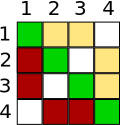
\includegraphics[width=0.32\textwidth]{example_2_matrix}
        }%
        \subfigure[Un DAG à 4 cellules]{%
          \label{fig:example_3_dag}
          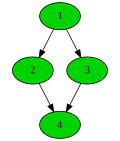
\includegraphics[width=0.32\textwidth]{example_3_dag}
        }%
    \end{center}
    \caption{Trois représentations d'un réservoir. Les éléments en rouge dans la matrice déterminent les dépendances dans le graphe de tâches.}
    \label{fig:exemple_3_dag}
\end{figure}

\begin{algorithm}
  \KwData{$M$ : matrice de dimension $n$}
  \For{$i = 2$ {\bf à} $n$} {
    \For{$k = 1$ {\bf à} $i - 1$ {\bf et} $M_{ik} != 0$} { \label{algo:ilu0:task_begin}
      $M_{ik} = M_{ik} / M_{kk}$ \label{algo:ilu0:dep}\\
      \For{$j = k + 1$ {\bf à} $n$ {\bf et} $M_{ij} != 0$} {
        $M_{ij} = M_{ij} - M_{ik}M_{kj}$ \\
      }
    } \label{algo:ilu0:task_end}
  }
  \caption{Factorisation ILU(0) sur place.}
  \label{algo:ilu0}
\end{algorithm}


En résumé, le parallélisme de l'algorithme ILU peut se représenter sous la forme d'un graphe de tâches.
%
Chaque tâche représentant la factorisation d'une ligne... ce qui est bien petit.
%
En fait, la plupart des runtimes mettront plus de temps à ordonnancer la tâche que la tâche mettra à factoriser une ligne.


Les problèmes rencontrés pour paralléliser la factorisation incomplète d'une matrice creuse, ainsi que les résolutions triangulaires associées, sont des problèmes qui représentent bien la difficulté que l'on peut rencontrer avec une parallélisation à grain fin.
%
La description à grain fin de ces algorithmes est naturelle, mais en pratique, une simple parallélisation utilisant des ordonnanceurs répandus, tels que Intel TBB ou OpenMP, ne donnera pas de bonnes performances à cause du faible coût de calcul d'une tâche.
%
On appelle cela le problème de granularité.
%
Pour résoudre ce problème, les tâches doivent devenir plus grosses, nous devons factoriser plusieurs lignes à l'intérieur d'une tâche.
%
Mais le choix de ces lignes n'est pas trivial, il faut limiter l'impact sur le parallélisme et ne pas changer le résultat final.
%
Une méthode générique a été développée durant la thèse et sera expliquée plus loin dans ce document.
%
De plus, l'ordre de factorisation des lignes de la matrice aura une influence sur les performances.
%
En fonction du nombre de variables primaires, nous avons entre 24~\% et 450~\% de temps de factorisation en plus par rapport au temps de factorisation optimal (Tab.~\ref{tab:facto_order}).
%
La factorisation des lignes de la matrice avec un parcourt linéaire des indices donne les meilleurs performances.
%
Il est donc primordial d'agréger des tâches qui factorisent des lignes consécutives de la matrice.

%   (-_-)   %
\begin{center}
  \begin{tabular}{|r|c|c|c|}
    \hline
    Nombre de variables primaire & Temps avec un parcourt & Temps avec un parcourt & Pourcentage de temps\\
    & linéaire des indices (s) & non linéaire des indices (s) & en plus \\
    \hline
    1 & 0.16 & 0.88 & 450~\% \\
    \hline
    3 & 0.43 & 1.43 & 230~\% \\
    \hline
    8 & 3.95 & 5.18 & 24~\% \\
    \hline
  \end{tabular}
  \captionof{table}{Différence de temps d'une factorisation d'une matrice de 1 million de lignes en fonction de la méthode de parcours des indices de lignes.}
  \label{tab:facto_order}
\end{center}




Il existe des travaux de recherche dont le but est aussi d'exploiter le parallélisme de l'algorithme ILU.
%
En changeant la numérotation des cellules, on peut modifier la structure de la matrice ce qui aura pour effet de changer la factorisation.
%
Une renumérotation rouge-noire permet de factoriser parallèlement la moitié des lignes de la matrice dans un premier temps, puis la seconde moitié des lignes dans un second temps.
%
Cette technique offre énormément de parallélisme mais aura un impact négatif sur la convergence\cite{red_black_ilu}.
%
Plus récemment, une autre méthode a été développée permettant de factoriser tous les éléments de la matrice en parallèle tout en gardant une numérotation naturelle.
%
L'opération de factorisation parallèle est appelé {\em sweep} et doit être effectuée plusieurs fois\cite{chow2014fine}.
%
En moyenne 3 sweeps suffisent à obtenir un résultat proche de la factorisation incomplète.
%
La convergence n'est donc que faiblement dégradée, mais il faut prendre en compte que 3 sweeps ont été nécessaires et il a donc fallu faire 3 fois plus d'opérations qu'une factorisation ILU classique.

%   (-_-)   %
\begin{figure}[!h]
     \begin{center}
        \subfigure[Exemple de graphe de tâche obtenu avec une numérotation naturelle.]{%
          \label{fig:DAG_natural}
          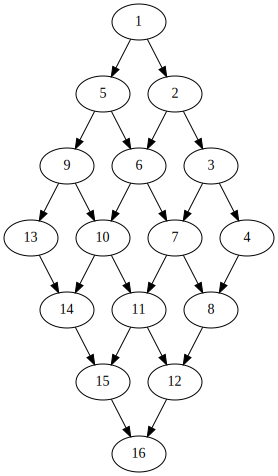
\includegraphics[width=0.33\textwidth]{DAG_natural}
        }%
        \subfigure[Exemple de graphe de tâche obtenu avec une numérotation rouge-noire.]{%
          \label{fig:DAG_redblack}
          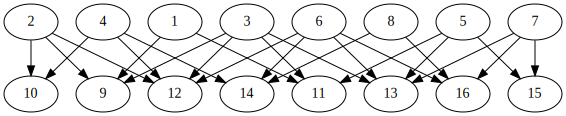
\includegraphics[width=0.66\textwidth]{DAG_redblack}
        }%
    \end{center}
    \caption{Différence de parallélisme en fonction de la numérotation choisie. La figure \ref{fig:matrix_ordering} représente les matrices associées.}
    \label{fig:DAG_ordering}
\end{figure}

%-------------------------------
%+++++++++++++++++++++++++++++++

%+++++++++++++++++++++++++++++++
\section{Pourquoi la granularité est si importante?}
%-------------------------------
\subsection{Parallelism vs overhead}
A task-based runtime need to dispatch tasks all over the available computational cores.
%
But this action isn't completely free, some operations need to be done by the scheduler and depends on its implementation.
%
Generally more the runtime is complex, more it will spend time to dispatch tasks.
%
A very simple runtime could be composed of a shared queue, in which tasks are inserted when a core can execute them.
%
This queue must be thread safe since every thread will enqueue/dequeue tasks at the same time.
%
Unfortunately, even this type of runtime have an overhead when it enqueue/dequeue a task.
%
This overhead can be negligible if the time spend in the task is much higher than the overhead.
%
But with a fine-grain parallelism, this overhead is far to be considerate as negligible and the programmer needs to deal with it.
%
Even a static scheduler has overhead, since all tasks are distributed over all cores, the scheduler needs to check if all dependencies of the task are satisfied.
%
This could be do more or less efficiently but in all case we lost the dynamic load balancing aspect of a dynamic scheduler.


Increasing the grain size of tasks in a program is a solution, but it could also reduce the possibilities of parallelism and load balancing provide by the runtime.
%
Parallelism and load balancing are linked, runtime need to have enough parallelism to achieve a good load balancing.
%
So, most of the time, finding the perfect grain size is painful.
%
If the grain size is too big, the runtime cannot fairly balance the computation over all cores of the processor.
%
But on the contrary, if the grain size is too small, the overhead of the runtime kills performances.


Several related works have been conducted in the past to address the issue of adapting the task grain size to the amount of available computing units.
%
Many related works partially address this grain size issue by promoting cache-oblivious techniques for a specific class of
applications such as recursive, divide-and-conquer codes or recursively partitioned loops~\cite{unifieddataflow,Intel::TBB,Cilk,xkaapi,taskscomparison}.
%
Works such as the SCOOPP framework~\cite{scoopp} provides means for the applications to control the task grain size.
%
However, the grain size selection issue is still up to the application programmer.


On the theoretical side, general task scheduling has been heavily studied for a long time now~\cite{Khan94acomparison,heft}.
%
Works on task grain adaptiveness have been scarcer, but do exist.

%-------------------------------
\subsection{Current solutions}
The granularity problem of task based programming is well know problem, it has been studied for a long time.
%
Some task based runtimes tried to solve this problem with different approach.
%
For example, X-Kaapi introduces the concept of splittable task, when a worker switches to the idle state, it emits a steal request to another worker.
%
The other workers, in working state, need to check regularly if they receive a steal request.
%
Then the work is split into two pieces, the split function needs to be written by the programmer, it's not automatic.
%
The split function can be trivial in case of parallel for loop or in case of tree task flow.
%
But in general case, it's not always possible to separate a DAG into two totally independent DAG.


Another possible approach, as given by Capsules\cite{capsules}, requires the user to define several grain sizes.
%
The runtime then chooses which grain best matches the current situation.
%
The application programmer must therefore design his/her application while having these multiple granularity levels in mind, which may prove difficult to realize or express in an abstract way in the code.

%+++++++++++++++++++++++++++++++


%+++++++++++++++++++++++++++++++
\section{Proposition de solution à notre problème de granularité}
%-------------------------------
\subsection{Taggre : un cadriciel pour agréger des tâches}
Nous avons pour but de garder la façon naturelle de décrire le parallélisme dans les noyaux d'algèbre linéaire creuse.
%
Malheureusement, cette granularité est trop fine, l'ordonnanceur de tâches met plus de temps à choisir quel sera le processeur qui traitera la tâche que le processeur met à traiter la tâche.
%
Pour obtenir des performances raisonnables, nous devons augmenter la granularité de la description du problème.
%
Pour cela, nous proposons de créer des groupes de tâches, de considérer chaque groupe comme une seule tâche et d'ordonnancer tous ces groupes en tant que graphe de tâches pour ainsi réduire le surcoût lié à l'ordonnanceur.
%
Au final, nous obtenons un graphe composé de moins de tâches, mais il faut faire attention à ne pas trop réduire le parallélisme fourni par le graphe.
%
Pour un graphe issu de la simulation de réservoir, nous connaissons déjà une solution efficace capable de répondre à une partie du problème.
%
Dans le cas d'un cube 3D avec une numérotation naturelle, nous pouvons changer la granularité en factorisant des groupes de lignes correspondant à une arête du cube.
%
Malheureusement, cette méthode ne fonctionne qu'avec une seule numérotation et nous impose de connaître la taille du cube.
%
Nous avons donc cherché une méthode pouvant s'appliquer à n'importe quel graphe de tâches.


En partant de la représentation la plus fine sous forme de graphe de tâches du parallélisme, nous avons besoin de calculer un nouveau graphe plus grossier avec moins de tâches.
%
La principale difficulté est de garder la propriété {\em acyclique} du graphe, car la présence d'un cycle introduirait un inter-blocage dans l'ordonnancement du graphe (Fig.~\ref{fig:agg_invalid}).
%
L'autre difficulté est de maintenir assez de parallélisme pour pouvoir être capable d'utiliser au mieux les capacités de la machine.


\begin{figure}[!h]
     \begin{center}
        \subfigure[Agrégation invalide]{
          \label{fig:agg_invalid}
          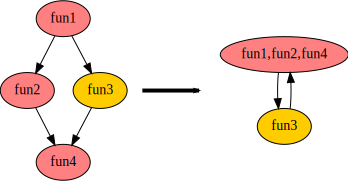
\includegraphics[width=0.4\textwidth]{agg_invalid}
        }
        ~
        \subfigure[Agrégation valide]{
          \label{fig:agg_valid}
          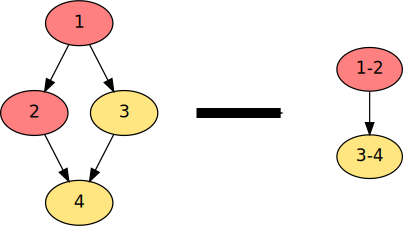
\includegraphics[width=0.4\textwidth]{agg_valid}
        }
    \end{center}
    \caption{Exemple de deux agrégations, le résultat de \ref{fig:agg_invalid} ne peut pas être ordonnancé à cause du cycle. Le résultat de \ref{fig:agg_valid} peut être ordonnancé, mais il n'y a aucun parallélisme à exploiter.}
    \label{fig:agg_basic}
\end{figure}


En premier lieu, nous avons développé une nouvelle interface de programmation en C++, cette interface reprend de Intel TBB le concept d'un objet {\em Tâche} contenant la fonction à exécuter.
%
\`A cela, nous avons ajouté la description des dépendances dans cet objet.
%
Cette interface nous permet de décrire un graphe de tâches complet et de choisir parmi plusieurs ordonnanceurs celui qui ordonnancera le graphe.
%
Avec cette interface, nous pouvons faire des modifications sur le graphe et le rendre plus grossier.
%
Nous avons appelé cette interface Taggre.
%
Grâce à l'utilisation d'heuristiques décrites plus loin dans le manuscrit, un programme parallèle peut continuer de décrire son parallélisme de façon naturelle, sans se soucier de la granularité.
%
Taggre s'occupera ensuite de faire le travail nécessaire pour rendre ce graphe assez grossier pour qu'un ordonnanceur puisse l'ordonnancer efficacement (Fig.~\ref{fig:coarsening}).
%   (-_-)   %
\begin{figure}
  \centering
  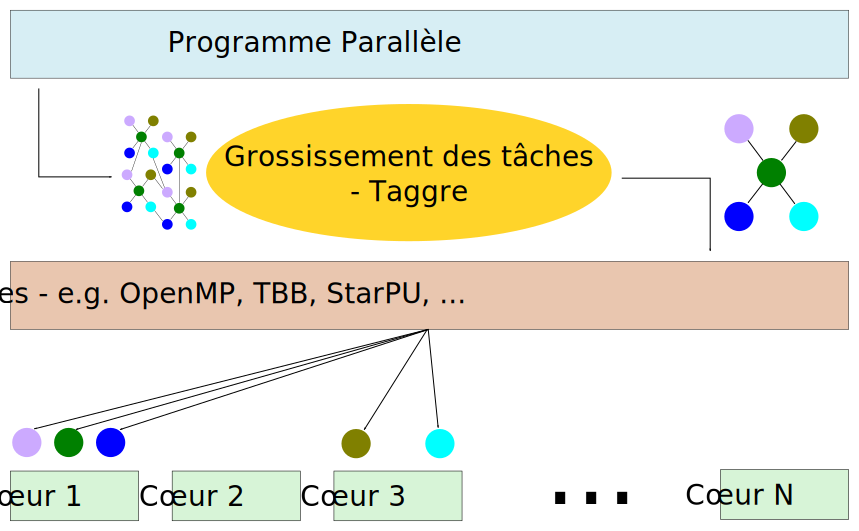
\includegraphics[width=0.8\textwidth]{coarsening}
  \caption{Le programme parallèle fournit un graphe de tâches à Taggre. Taggre modifie le graphe. Taggre fournit le graphe à l'ordonnanceur. Le processus d'agrégation est totalement transparent pour l'ordonnanceur.}
  \label{fig:coarsening}
\end{figure}


\lstinputlisting[inputencoding=utf8/latin1,frame=single,float=t,caption=Exemple d'utilisation de Taggre,label=taggrecpp]{src/taggre.cpp}



Dans un premier temps, le programmeur crée les noeuds du graphe, ces noeuds correspondent aux tâches fines du problème.
%
Pour chaque noeud créé le programmeur reçoit un identifiant de noeud.
%
Puis le programmeur déclare les arêtes du graphe en utilisant les identifiants des noeuds.
%
Maintenant que le graphe de tâches fines est connu, Taggre peut travailler à grossir le grain.
%
La méthode {\em coarse} effectuera le travail avec les paramètres que nous expliquerons plus loin dans le manuscrit.
%
Nous avons donc un nouveau graphe composé de tâches grossières, mais ces tâches n'ont toujours pas de code à exécuter.
%
Pour définir le code à exécuter, le programmeur doit appeler la méthode {\em setup} avec comme paramètre une fonction qui créera les tâches grossières.
%
Cette fonction connaîtra les tâches fines associées à la tâche grossière et pourra ainsi optimiser le code en fonction du nombre et des types de tâches agrégées.
%
Finalement, le programmeur exécutera toutes les tâches du graphe avec la méthode {\em run}.
%
Il a aussi la possibilité d'utiliser une fonction générique avec la méthode {\em run\_function} (voir Listing~\ref{taggrecpp}).

%-------------------------------
\subsection{Les opérateurs d'agrégations}
Nous appelons {\em opérateurs d'agrégations} les différentes heuristiques utilisés pas Taggre pour grossir un graphe de tâches.
%
Ces heuristiques ont pour règle de garder la propriété acyclique du graphe de tâches.
%
Quatre heuristiques ont été crées, chaque opérateur s'occupe de résoudre un problème spécifique et aucun d'entre eux ne peux créer de cycle.
%
La création d'un cycle lors d'une agrégation intervient lorsque l'on crée un groupe de tâche dans lequel deux des tâches ont une dépendance indirecte, symbolisé par un chemin dans le graphe, et qu'au moins une des tâches de ce chemin n'appartient pas au groupe.


%Pour évaluer l'amélioration apportée par chaque heuristique, nous avons intégré dans Taggre un simulateur minimal qui estimera le temps d'ordonnancement du graphe.
% Les résultats du simulateur minimal ne sont pas bons
%Cette estimation est essentielle dans la mesure où elle permet de mesurer le parallélisme restant pouvant être extrait du graphe grossier.

On pourrait se poser la question de l'utilisation d'un partitionneur de graphe comme opérateur d'agrégation.
%
En effet, les partitionneurs de graphe essaient de créer des groupes de noeud proche spatialement.
%
Si nous prenons en compte ce seul paramètre, ils feraient des opérateurs de très bonne qualité.
%
Malheureusement, les partitionneurs ne travaillent que sur des graphes non orientés.
%
Le résultat de ces opérateurs serait donc inutilisable parce que les graphes obtenus pourraient être composés de cycles.

%-------------------------------
\subsubsection{Séquentiel}
L'opérateur séquentiel, aussi abrégé {\em S} dans Taggre, est un opérateur très simple.
%
Son but est de fusionner les tâches qui n'apportent pas de parallélisme, elles ne font qu'ajouter du surcoût d'ordonnancement au temps total de la simulation.
%
En agrégeant ces tâches ensemble, on ne perd pas de parallélisme et on économise le temps d'ordonnancement des tâches.
%
On peut reconnaître un groupe de deux tâches séquentielles par le fait qu'une des tâches n'a qu'un seul successeur et l'autre tâche n'a qu'un seul prédécesseur (Fig.~\ref{fig:algo_S}, Algo.~\ref{algo:algo_S}).


%   (-_-)   %
\begin{figure}[!h]
  \centering
  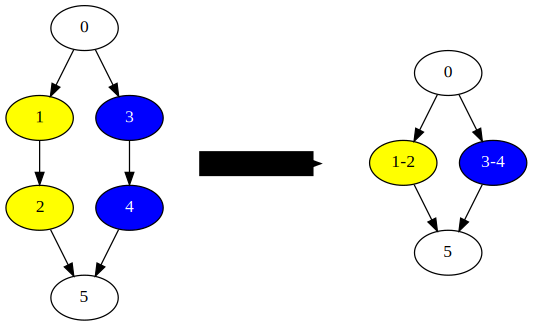
\includegraphics[width=0.6\textwidth]{algo_S}
  \caption{Exemple d'agrégation par l'opérateur séquentiel.}
  \label{fig:algo_S}
\end{figure}

\begin{algorithm}
  \KwData{DAG}
  {\sc Taches} = liste vide \\
  mettre les tâches de DAG dans {\sc Taches} \\
  \While{{\sc Taches} n'est pas vide} {
    {\sc T1} = retirer le premier de {\sc Taches} \\
    \If{Le nombre de successeurs de {\sc T1} == 1} {
      {\sc T2} = premier successeur de {\sc T1} \\
      \If{Le nombre de prédécesseurs de {\sc T2} == 1} {
        {\sc T2} devient {\sc T1} union {\sc T2}\\
      }
    }
  }
  \caption{Algorithme de l'opérateur séquentiel.}
  \label{algo:algo_S}
\end{algorithm}

L'opérateur S ne détruit pas de parallélisme et peu potentiellement réduire le nombre de tâches.
%
En partant de ce postulat, on pourrait penser appliquer cet opérateur systématiquement après chaque agrégation.
%
Mais il faut garder en tête que créer des tâches de granularité trop différentes peut impacter les politiques d'ordonnancement de tâches.
%
Certains ordonnanceurs pourraient utiliser ces tâches en temps que tâches {\em tampons} pour les parties du graphe où il manque du parallélisme.

\subsubsection{Front}
L'opération front, abrégé {\em F} dans Taggre, va limiter le nombre de tâche disponible au même moment dans l'odonnanceur.
%
Un graphe fournissant énormément de parallélisme par rapport au nombre de coeur disponible n'aura pas forcément un meilleur équilibrage de charge par rapport à un graphe offrant moins de parallélisme.
%
Donc à part congestionner les structures de données servant à maintenir à jour les tâches prêtes à être ordonnancer, il n'est pas nécessaire d'avoir trop de parallélisme dans un graphe.
%
Le parallélisme d'un graphe peut être corréler à sa largeur.
%
En effet, avec un nombre illimité de coeur de calcul, on peut exploiter au mieux la même nombre de coeur que la largeur du graphe.
%
L'algorithme de l'opérateur F consiste à parcourir le graphe par hauteur et de limiter le nombre de tâches par hauteur à un paramètre donné par le programmeur (Fig.~\ref{fig:algo_F2}).
%
Seul les tâches qui ont la même hauteur sont agrégés ensemble, il n'y a donc aucun risque de créer un cycle.
%   (-_-)   %
\begin{figure}[t!]
  \centering
  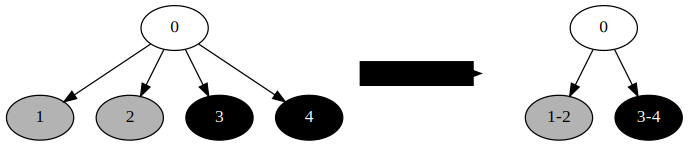
\includegraphics[width=0.7\textwidth]{algo_F2}
  \caption{Exemple d'agrégation avec l'opérateur F et le paramètre 2.}
  \label{fig:algo_F2}
\end{figure}


\subsubsection{Dézoomé}
Je pense qu'il s'agit de l'opérateur le plus intéressant parce qu'il permet d'effectuer des agrégations assez génériques et souvent efficace.
%
Abrégé {\em D} dans Taggre, cet opérateur essaye de créer des groupes de tâches proche spacialement, un peu à la manière d'un partitionneur de graphe.
%
Le nom {\em dézoomé} provient du fait que la structure globale du graphe n'a pas beaucoup changée pendant l'agrégation mais que le nombre de tâches a lui considérablement diminué.
%
Dans les meilleurs cas le nombre de tâches peut être divisé par le paramètre donné par le programmeur (Fig.~\ref{fig:algo_D4}).
%
L'algorithme \ref{algo:algo_D} permet d'implémenter l'opérateur dézoomé tout en assurant l'absence de création de cycle.
%   (-_-)   %
\begin{figure}[t!]
  \centering
  \includegraphics[width=0.7\textwidth]{algo_D4}
  \caption{Exemple d'utilisation de l'opérateur D avec le paramètre 4. Le nombre total de tâche a bien été divisé par 4.}
  \label{fig:algo_D4}
\end{figure}

\subsubsection{Cube ou continuation}
Cet opérateur a été créé pour être une réponse efficace à nos problèmes.
%
Dans notre cas, le graphe à ordonnancer à exactement la même structure que le réservoir que nous souhaitons modéliser.
%
La plupart du temps, ce modèle sera un cube 3D.
%
En numérotation naturelle et avec un modèle 3D, une bonne agrégation consiste à agréger toutes les tâches d'un axe qui ont les mêmes coordonnées sur les deux autres axes.
%
Cela correspond à {\em aplatir} notre modèle 3D en un modèle 2D (Fig.~\ref{fig:cube5_algo_C}).
%
Par exemple, un cube de 5 éléments de coté, soit 125 tâches, sera transformé en un carré de 5 éléments de coté, soit 25 tâches.


%   (-_-)   %
\begin{figure}
  \centering
  \includegraphics[width=\textwidth]{cube5_operator_c}
  \caption{Exemple d'utilisation de l'opérateur C sur un cube 5x5x5.}
  \label{fig:cube5_algo_C}
\end{figure}


%   (-_-)   %
\begin{figure}
  \centering
  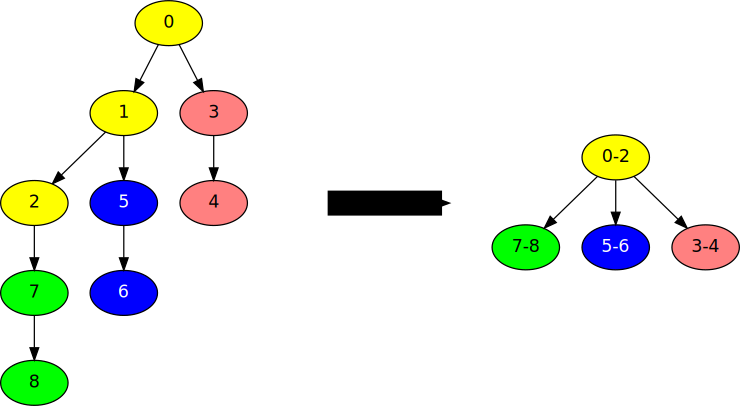
\includegraphics[width=0.8\textwidth]{algo_3}
  \caption{Exemple d'utilisation de l'opérateur C.}
  \label{fig:algo_C}
\end{figure}


Comme pour les autres opérateurs, nous devons vérifier qu'aucun cycle ne sera créé.
%
Pour fonctionner, cet opérateur a besoin que le programmeur attribue un nombre unique à chaque tâche et ainsi avoir un ordre strict sur les tâches.
%
Dans notre cas on va utiliser la numérotation naturelle des cellules.
%
Puis l'opérateur agrégera ensemble les tâches ayant des nombres qui se suivent ainsi qu'une dépendance entre les tâches.
%
Par exemple sur la figure \ref{fig:algo_C} les tâches 2 et 3 ont des nombres consécutifs mais n'ont pas de dépendance entre elles, elles ne seront donc pas agrégées ensemble.


Ajoutons un prédicat à l'algorithme : pour pouvoir utiliser cet algorithme, il faut absolument que pour chaque tâche $i$, l'indice associé à la tâche $i$ soit strictement inférieur aux indices associés aux successeurs de la tâche $i$.
%
Dans le cas d'une factorisation ILU, ce prédicat est toujours vérifié.
%
Dans le cas général, il nous permet de s'assurer qu'aucun cycle ne sera créé.
%
En effet, pour créer un cycle avec cet algorithme, il faudrait qu'il existe un chemin entre deux tâches agrégées qui passe par une autre tâche non agrégée.
%
Or, pour agréger une tâche avec une autre, il faut que la différence de leurs indices soit exactement la différence minimale possible dans le graphe.
%
Donc, en prenant en compte le prédicat, si nous agrégeons une tâche T1 avec son successeur T2, il ne peut pas exister de chemin en T1 et T2 passant par une autre tâche.


\begin{algorithm}
  \KwData{DAG}
  {\sc Pas} = Infini \\
  \For{chaque tâche {\sc T1} de DAG} {
    \For{chaque successeurs {\sc T2} de {\sc T1}} {
      \If{indice de {\sc T2} $<=$ indice de {\sc T1}} {
        \Return agrégation impossible
      }

      \If{indice de {\sc T2} - indice de {\sc T1} $<$ {\sc Pas}} {
        {\sc Pas} = indice de {\sc T2} - indice de {\sc T1}
      }
    }
  }

  \For{chaque tâche {\sc T1} de DAG} {
    \For{chaque successeurs {\sc T2} de {\sc T1}} {
      \If{indice de {\sc T2} == indice de {\sc T1} + {\sc Pas}} {
        {\sc T1} devient {\sc T1} union {\sc T2}
      }
    }
  }
  \caption{Algorithme de l'opérateur continuation.}
  \label{algo:algo_C}
\end{algorithm}

%% Dans le cas d'un graphe représentant un cube 3D, cet opérateur fonctionne très bien.
%% %
%% Par contre, dans le cas d'un graphe représentant un carré, il est nécessaire de modifier cette algorithme pour limiter la taille des agrégats tout en optimisant

%-------------------------------
\subsection{Exemples de stratégies}
\url{http://view.eecs.berkeley.edu/wiki/Dwarf_Mine}

Le choix des opérateurs dans Taggre se fait à l'appréciation du programmeur.
%
Les 13 nains de Berkeley est une méthode de classification des problèmes suivant leurs motifs de calculs et de communication.
%
On peut essayer de voir si Taggre peut répondre aux 13 problèmes et si c'est le cas quelle serai la stratégie d'agrégation à utiliser.

\subsubsection{Algèbre linéaire dense}
Les graphes utilisés en algèbre linéaire dense sont très régulier.
%
Une grande partie des optimisations de graphe peut être faite statiquement dans le code.
%
L'utilisation de Taggre reste toutefois possible, mais donnera des résultats moins bon.
%
L'opérateur D fonctionne très bien avec les problèmes réguliers.
%
Mais le plus efficace serai d'écrire un opérateur qui cherche des motifs pour les agréger en une seule tâche.


\subsubsection{Algèbre linéaire creuse}
Taggre a été conçu pour répondre aux problèmes de l'algèbre linéaire creuse.
%
Les techniques d'agrégations dépendront du problème à résoudre.
%
Dans notre cas, nous avons des modèles 3D, nous allons donc utiliser l'opérateur C.
%
Si le graphe n'est toujours pas assez grossier, nous pouvons ajouter l'opérateur D avec un paramètre assez petit.
%
Dans d'autre cas, il est nécessaire d'analyser le graphe mais généralement l'opérateur D avec un paramètre assez gros fonctionne.



\subsubsection{Méthodes spectrales}
Les méthodes spectrales sont composées de plusieurs paliers, les tâches d'un même palier sont indépendantes.
%
Les dépendances entre les paliers sont croisées.
%
L'opérateur F avec comme paramètre 2 à 3 fois le nombre de threads devrait limiter le parallélisme sans toutefois trop impacter l'équilibrage de charge.



\subsubsection{Méthodes N-Body}
Ici, il s'agit de simuler un ensemble de particules qui se déplacent.
%
Il n'y a pas de graphe statique de tâches, Taggre n'est pas efficace pour ce genre de méthodes.



\subsubsection{Grilles structurées}
Le problème de parallélisation des problèmes avec des grilles structurées peut se résoudre avec du parallélisme de boucle.
%
\'A chaque itération, chaque cellule est mise à jour en fonction des cellules adjacentes.
%
Si nous souhaitons utiliser Taggre, nous pouvons utiliser l'opérateur F pour grossir le grain de calcul.


\subsubsection{Grilles non-structurées}
Les solutions à ce problème sont les mêmes que pour les grilles structurées.
%
Il vaut mieux utiliser du parallélisme de boucle avec un ordonnanceur dynamique pour avec un bon équilibrage de charge.
%
Avec Taggre, il faut définir le poids de chaque tâche et utiliser l'opérateur F qui formera des tâches plus grossières de même poids.


\subsubsection{MapReduce}
Les problèmes de type MapReduce se parallélisent très bien à condition que la fonction de distribution soit correcte.
%
Il n'y a donc aucun intérêt à utiliser Taggre.



\subsubsection{Logique combinatoire}
Il s'agit de parallélisme pouvant seulement être résolu au moment de la conception des processeurs.
%
Le parallélisme est vraiment trop fin, Taggre ne peut rien faire.


\subsubsection{Graph Traversal}
Il n'a pas de graphe de tâches, les étapes sont totalement séquentielles.


\subsubsection{Dynamic Programming}
Le problème se présente sous la forme d'un arbre.
%
Il faut donc utiliser l'opérateur F suivi de l'opérateur S.


\subsubsection{Backtrack and Branch-and-Bound}
Le graphe n'est pas connu à l'avance, il est impossible d'utiliser Taggre.


\subsubsection{Graphical Models}
Il n'a pas de graphe de tâches, les étapes sont totalement séquentielles.


\subsubsection{Finite State Machines}
Les machines à états sont composées de graphes directes, mais ces graphes peuvent contenir des cycles.

%+++++++++++++++++++++++++++++++




%+++++++++++++++++++++++++++++++
\section{Résultats}
%-------------------------------
\subsection{Amélioration de la factorisation et de la résolution triangulaire}
Dans un premier temps, nous allons nous consacrer à l'amélioration de la parallélisation de la factorisation ILU(k).
%
Chaque tâche du DAG représente la factorisation d'une ligne de la matrice.
%
Cette granularité est trop fine, mais c'est voulu, elle représente la granularité que nous obtenons en décrivant naturellement le maximum  de parallélisme que nous pouvons exploiter.
%
Nous avons choisi de simuler deux réservoirs, un cube généré de taille 80 cellules de côté et le réservoir SPE10.
%
Dans le cas du cube, il est possible de choisir le nombre de variables primaires utilisées dans le calcul.
%
Pour rappel, le nombre de variables primaires correspond au nombre de composants simulés.
%
Chaque entrée non-nulle de la matrice correspond à l'interaction entre 2 cellules et sera composée d'une petite matrice dense $Npri*Npri$ avec $Npri$ le nombre de variables primaires.
%
Nous avons choisi de simuler le cube avec 1 variable primaire, 3 variables primaires (modèle {\em black-oil}) et 8 variables primaires (modèle {\em compositionnel}).
%
Pour le réservoir SPE10, c'est un cas {\em black-oil} à 3 variables primaires.
%
Au final nous avons donc 4 matrices différentes.
%
Nous ne faisons pas varier la taille du cube car les résultats obtenus avec des cubes générés de tailles raisonnablement différentes sont équivalents.


\subsubsection{Sans agrégation}
Nous avons utilisé OpenMP pour tester la parallélisation à grain fin sans agrégation.
%
OpenMP n'ayant pas de gestion de dépendances entre les tâches, nous utiliserons un système de décrémentation atomique.
%
Comme le montre les résultats de la figure~\ref{fig:res_facto_no_agg}, le nombre de variables primaires a une importance considérable sur les performances que nous obtenons.
%
L'utilisation de 2 threads n'est viable que dans le cas où nous utilisons 8 variables primaires.
%
Dans les autres cas, même en utilisant 4 threads, nous perdons du temps.
%
Ici, le nombre de variables primaires va définir le nombre d'opérations faites par ligne de la matrice, donc plus ce nombre est grand, plus il y aura de travail à faire.
%
Ces résultats confirment notre problème de granularité.
%
Au final, avec l'utilisation des 12 coeurs de calcul de la machine, nous obtenons des accélérations plutôt décevant, par exemple, pour les cas à 3 variables primaires, le code tourne environ 2,5 fois plus vite que la version séquentielle mais il utilise 12 fois plus de puissance de calcul.


%   (-_-)   %
\begin{figure}[!h]
  \centering
  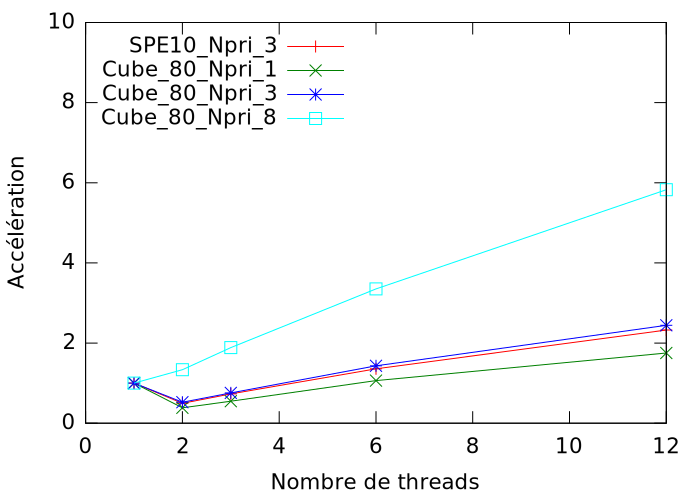
\includegraphics[width=0.7\textwidth]{res_facto_no_agg}
  \caption{Performance de la factorisation sur 12 coeurs sans utiliser Taggre.}
  \label{fig:res_facto_no_agg}
\end{figure}




\subsubsection{Avec l'opérateur F}
Dans un premier temps, nous allons appliquer l'opérateur F avec le paramètre 36.
%
Cet opérateur va donc limiter la largeur du graphe pour qu'il y ait au plus 36 tâches par hauteur du graphe.
%
Nous réduisons donc le parallélisme mais nous réduisons aussi le nombre de tâches, on divise par 62 le nombre de tâches pour un cube de 80 de côté, nous passons de 512000 tâches à 8223 tâches.
%
Pour le cas SPE10, le nombre de tâches passe de 1094435 à 12912 soit 84 fois moins de tâches.
%
La figure~\ref{fig:res_facto_f36} nous montre une amélioration du temps de factorisation quand le nombre de variables primaires est faible.
%
Cela vient du fait que le surcoût d'ordonnancement de la tâche est du même ordre de grandeur que le temps de calcul de la tâche.
%
Avec 3 variables primaires, la factorisation est 30~\% plus rapide.
%
Avec 1 variable primaire, le temps de factorisation est divisé par 2.
%
Dans le cas où le nombre de variables primaires est élevé, il n'y a pas beaucoup d'amélioration (6~\%).
%
Ici, cet opérateur ne permet pas d'optimiser les accès mémoire cache, seul le surcoût d'ordonnancement est réduit.


%   (-_-)   %
\begin{figure}[!h]
  \centering
  \includegraphics[width=0.7\textwidth]{res_facto_f36}
  \caption{Performance de la factorisation sur 12 coeurs avec Taggre F(36).}
  \label{fig:res_facto_f36}
\end{figure}





\subsubsection{Avec l'opérateur D}
Essayons maintenant l'opérateur D avec le paramètre 8.
%
Cet opérateur va essayer de créer des groupes de 8 tâches assez proches dans le graphe.
%
Nous allons donc diviser par 8 le nombre de tâches, passant ainsi de 512000 tâches à 64000 tâches.
%
Ce qui peut paraître peu mais cette valeur a été choisie empiriquement parmi un ensemble de valeurs.
%
Les autres valeurs donnent des résultats légèrement moins bons, par exemple le paramètre 4 offre une accélération de 3,35, tandis que le paramètre 12 offre 3,55 et finalement le paramètre 8 offre une accélération de 3,72.
%
Comparé à l'opérateur F, il y a très peu d'amélioration quand le nombre de variables primaires est faible (Fig.~\ref{fig:res_facto_d8}).
%
Par contre, avec 8 variables primaires, on obtient un gain de performance qui est dû à une meilleure utilisation des caches, surtout du cache L2 avec une diminution de 10\% des défauts de cache.

%   (-_-)   %
\begin{figure}[!h]
  \centering
  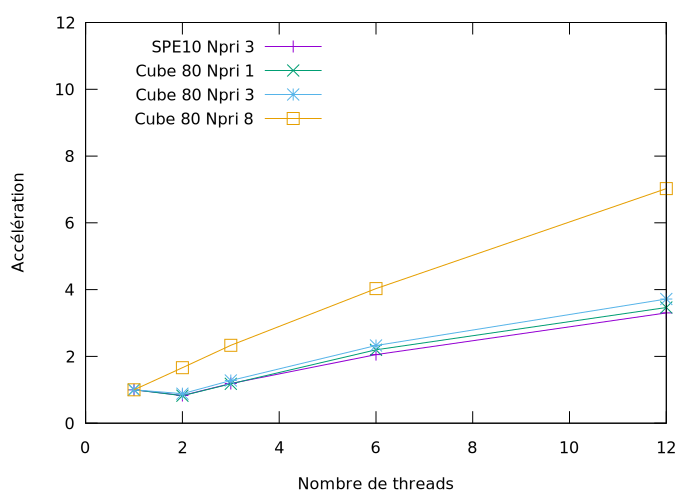
\includegraphics[width=0.7\textwidth]{res_facto_d8}
  \caption{Performance de la factorisation sur 12 coeurs avec Taggre D(8).}
  \label{fig:res_facto_d8}
\end{figure}





\subsubsection{Avec l'opérateur C}
Les deux précédents opérateurs donnent déjà des résultats, mais nous pensons que le meilleur opérateur pour nos matrices reste l'opérateur C.
%
Il a l'avantage de réduire grandement le nombre de tâche comme l'opérateur F et il forme des groupes de tâches permettant une meilleure réusabilité des données en cache.
%
Par contre, il se pourrait que le parallélisme en pâtisse.
%
Comme le montre les résultats de la figure~\ref{fig:res_facto_c}, tous les cas tests sont améliorés.
%
Il y a bien deux grandes améliorations : la réduction du nombre de tâches et une meilleure réutilisation des caches.
%
Comme pour tous les opérateurs, il y a une réduction du nombre de tâches, mais dans ce cas la réduction est bien plus importante.
%
Par contre, l'amélioration des effets caches est bien meilleure que dans les autres opérateurs.
%
Cette amélioration est inexistante dans le cas de l'opérateur F, les tâches agrégées n'avaient pas une bonne réutilisabilité des données en cache.
%
Au contraire, l'opérateur D ne réduisait que de très peu le nombre de tâches mais améliorait la réutilisation des caches.
%
L'opérateur C offre donc le meilleur des deux opérateurs, il produit peu de tâches et en plus ces tâches réutilisent correctement les données en cache.
% L2 stats : F:1.10, D:0.96, C:0.87


%   (-_-)   %
\begin{figure}[!h]
  \centering
  \includegraphics[width=0.7\textwidth]{res_facto_c}
  \caption{Performance de la factorisation sur 12 coeurs avec Taggre C.}
  \label{fig:res_facto_c}
\end{figure}


\subsubsection{Avec plusieurs opérateurs}
Il est aussi possible de combiner plusieurs opérateurs, sur la figure~\ref{fig:res_facto_cd2} nous avons combiné l'opérateur C avec l'opérateur D(2).
%
On observe un très léger gain de performance quand on a une seule variable primaire, mais dans les autres cas on observe le contraire.
%
Malgré ces optimisations, nous n'atteignons pas une accélération parfaite, avec au mieux une accélération de 8,7 pour 12 coeurs.
%
Ce souci de performance est lié à l'architecture mémoire de la machine, nous donnerons plus d'explication dans la partie suivante de la thèse.

%   (-_-)   %
\begin{figure}[!h]
  \centering
  \includegraphics[width=0.7\textwidth]{res_facto_cd2}
  \caption{Performance de la factorisation sur 12 coeurs avec Taggre CD(2).}
  \label{fig:res_facto_cd2}
\end{figure}

\subsubsection{En résumé}


%   (-_-)   %
\begin{center}
  \begin{tabular}{|r|c|c|c|c|c|c|c|c|c|c|}
    \hline
    Type de  &  \multicolumn{5}{c|}{Accélération}  &  \multicolumn{5}{c|}{Nombre de tâches} \\
    matrice  &  \O & F(36) & D(8) & C & CD(2)  &  \O & F(36) & D(8) & C & CD(2)\\
    \hline
    Cube 80 Npri 1 & 1,75 & 3,39 & 3.46 & 5.65 & 5.73 & 512000  & 8223  & 64000  & 6400  & 3200 \\
    Cube 80 Npri 3 & 2,44 & 3,46 & 3.72 & 6.07 & 6.14 & 512000  & 8223  & 64000  & 6400  & 3200 \\
    Cube 80 Npri 8 & 5,83 & 6,17 & 7.02 & 8.58 & 8.48 & 512000  & 8223  & 64000  & 6400  & 3200 \\
    SPE10 Npri 3   & 2,32 & 3,52 & 3.30 & 6.65 & 6.73 & 1094435 & 12912 & 136938 & 36336 & 18373 \\
    \hline
  \end{tabular}
  \captionof{table}{Récapitulatif des résultats de la factorisation suivant les opérateurs appliqués.}
  \label{tab:facto_res}
\end{center}


\subsubsection{Résultats de la résolution triangulaire}
Essayons maintenant cette technique sur la partie résolution triangulaire du code.
%
Les performances sans agrégations sont bien en dessous de la partie factorisation (Fig.~\ref{fig:res_trsv_no_agg}).
%
Même en utilisant 12 threads, seule la version avec 8 variables primaires donne de meilleurs résultats que la version séquentielle.
%
Encore une fois il s'agit d'un problème de granularité, le graphe à ordonnancer est le même que pour la factorisation mais les tâches sont plus petites.


%   (-_-)   %
\begin{figure}[!h]
  \centering
  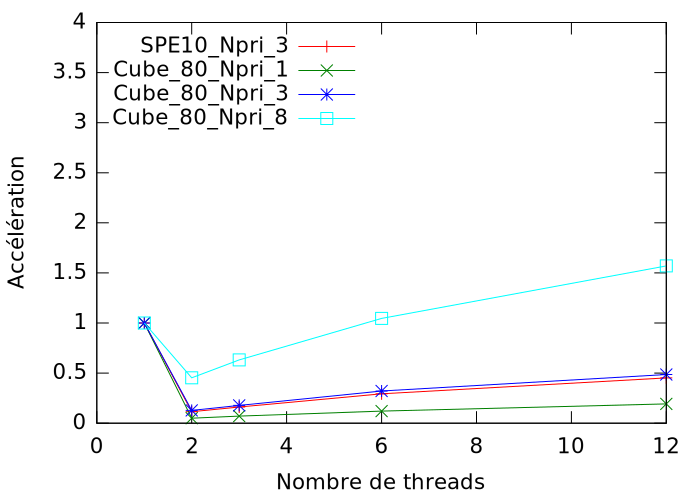
\includegraphics[width=0.7\textwidth]{res_trsv_no_agg}
  \caption{Performance de la résolution triangulaire sur 12 coeurs sans utiliser Taggre.}
  \label{fig:res_trsv_no_agg}
\end{figure}


Si nous regardons les résultats avec la meilleure agrégation que nous ayons, l'agrégation CD(2), on obtient des résultats légèrement meilleurs mais on n'est encore loin de l'accélération parfaite (Fig.~\ref{fig:res_trsv_cd2}).
%
On arrive ici au limite de notre méthode, la granularité n'est pas encore suffisante pour permettre d'obtenir de très bonnes performances.
%
Mais si nous augmentons encore la granularité, il n'y aura plus assez de parallélisme pour avoir un bon équilibrage de charge et le temps final sera supérieur.


%   (-_-)   %
\begin{figure}[!h]
  \centering
  \includegraphics[width=0.7\textwidth]{res_trsv_cd2}
  \caption{Performance de la résolution triangulaire sur 12 coeurs avec Taggre CD(2).}
  \label{fig:res_trsv_cd2}
\end{figure}


%% +---------------------------+-------------+-------------+-------------+------------+
%% |          Metric           |     Sum     |     Max     |     Min     |    Avg     |
%% +---------------------------+-------------+-------------+-------------+------------+
%% | Runtime (RDTSC) [s] STAT  |   1923.94   |   160.328   |   160.328   |  160.328   |
%% | Runtime unhalted [s] STAT |   1870.36   |   160.82    |   152.347   |  155.864   |
%% |     Clock [MHz] STAT      |   34528.4   |   2906.13   |   2850.24   |  2877.37   |
%% |         CPI STAT          |   1.03608   |   1.04174   |   1.02468   | 0.0863398  |
%% |  Data cache misses STAT   | 4.59444e+10 | 4.08753e+09 | 3.71715e+09 | 3.8287e+09 |
%% | Data cache miss rate STAT |   0.10934   | 0.00932521  | 0.00905509  | 0.0091117  |
%% +---------------------------+-------------+-------------+-------------+------------+
%% +---------------------------+-------------+-------------+-------------+-------------+
%% |          Metric           |     Sum     |     Max     |     Min     |     Avg     |
%% +---------------------------+-------------+-------------+-------------+-------------+
%% | Runtime (RDTSC) [s] STAT  |   2004.24   |   167.02    |   167.02    |   167.02    |
%% | Runtime unhalted [s] STAT |   2061.97   |   175.567   |   170.297   |   171.831   |
%% |     Clock [MHz] STAT      |   36151.6   |   3017.39   |   3008.02   |   3012.64   |
%% |         CPI STAT          |   1.14231   |   1.14711   |   1.13205   |  0.0951929  |
%% |  Data cache misses STAT   | 4.87067e+10 | 4.29088e+09 | 4.00937e+09 | 4.05889e+09 |
%% | Data cache miss rate STAT |  0.115926   | 0.00990628  | 0.00962271  | 0.00966052  |
%% +---------------------------+-------------+-------------+-------------+-------------+
%% +---------------------------+-------------+-------------+-------------+-------------+
%% |          Metric           |     Sum     |     Max     |     Min     |     Avg     |
%% +---------------------------+-------------+-------------+-------------+-------------+
%% | Runtime (RDTSC) [s] STAT  |   1640.85   |   136.737   |   136.737   |   136.737   |
%% | Runtime unhalted [s] STAT |   1686.77   |   144.388   |   138.353   |   140.564   |
%% |     Clock [MHz] STAT      |   36255.7   |   3046.34   |   2998.08   |   3021.31   |
%% |         CPI STAT          |  0.934931   |  0.937527   |  0.926718   |  0.0779109  |
%% |  Data cache misses STAT   | 3.85951e+10 | 3.43628e+09 | 3.14135e+09 | 3.21626e+09 |
%% | Data cache miss rate STAT |  0.0919074  | 0.00789712  | 0.00762214  | 0.00765895  |
%% +---------------------------+-------------+-------------+-------------+-------------+




%% +---------------------------+----------+-----------+-----------+-----------+
%% |          Metric           |   Sum    |    Max    |    Min    |    Avg    |
%% +---------------------------+----------+-----------+-----------+-----------+
%% | Runtime (RDTSC) [s] STAT  | 2013.52  |  167.794  |  167.794  |  167.794  |
%% | Runtime unhalted [s] STAT |  2049.5  |  173.386  |  167.781  |  170.792  |
%% |     Clock [MHz] STAT      | 35861.8  |  3005.94  |  2972.33  |  2988.48  |
%% |         CPI STAT          | 1.13698  |  1.14624  |  1.12814  | 0.0947487 |
%% |   L2 request rate STAT    | 0.139712 | 0.0119216 | 0.0115742 | 0.0116426 |
%% |     L2 miss rate STAT     | 0.154052 | 0.0129583 | 0.0127815 | 0.0128376 |
%% |    L2 miss ratio STAT     | 13.2323  |  1.10948  |  1.08696  |  1.10269  |
%% +---------------------------+----------+-----------+-----------+-----------+
%% +---------------------------+----------+-----------+-----------+-----------+
%% |          Metric           |   Sum    |    Max    |    Min    |    Avg    |
%% +---------------------------+----------+-----------+-----------+-----------+
%% | Runtime (RDTSC) [s] STAT  | 1966.96  |  163.913  |  163.913  |  163.913  |
%% | Runtime unhalted [s] STAT | 1886.06  |  158.261  |  156.494  |  157.172  |
%% |     Clock [MHz] STAT      | 34326.8  |  2883.42  |  2837.74  |  2860.57  |
%% |         CPI STAT          | 1.03718  |  1.06006  |  1.01601  | 0.0864318 |
%% |   L2 request rate STAT    | 0.152488 | 0.0130698 | 0.0125945 | 0.0127073 |
%% |     L2 miss rate STAT     | 0.14729  | 0.0125144 | 0.0121436 | 0.0122742 |
%% |    L2 miss ratio STAT     | 11.5912  | 0.970545  | 0.957504  | 0.965933  |
%% +---------------------------+----------+-----------+-----------+-----------+
%% +---------------------------+----------+-----------+-----------+-----------+
%% |          Metric           |   Sum    |    Max    |    Min    |    Avg    |
%% +---------------------------+----------+-----------+-----------+-----------+
%% | Runtime (RDTSC) [s] STAT  |  1652.6  |  137.716  |  137.716  |  137.716  |
%% | Runtime unhalted [s] STAT | 1694.79  |  142.824  |  140.196  |  141.233  |
%% |     Clock [MHz] STAT      | 36166.7  |  3035.99  |  2993.16  |  3013.9   |
%% |         CPI STAT          | 0.937105 | 0.962554  | 0.921956  | 0.0780921 |
%% |   L2 request rate STAT    | 0.158081 | 0.0134666 | 0.0131121 | 0.0131734 |
%% |     L2 miss rate STAT     | 0.138087 | 0.0116948 | 0.0114514 | 0.0115072 |
%% |    L2 miss ratio STAT     | 10.4823  |  0.87775  |  0.86843  | 0.873526  |
%% +---------------------------+----------+-----------+-----------+-----------+


%% +---------------------------+----------+-----------+---------+------------+
%% |          Metric           |   Sum    |    Max    |   Min   |    Avg     |
%% +---------------------------+----------+-----------+---------+------------+
%% | Runtime (RDTSC) [s] STAT  | 2014.07  |  167.839  | 167.839 |  167.839   |
%% | Runtime unhalted [s] STAT | 2045.66  |  172.625  | 168.205 |  170.471   |
%% |     Clock [MHz] STAT      | 35826.2  |  3000.16  | 2971.72 |  2985.52   |
%% |         CPI STAT          | 1.13743  |  1.14473  | 1.12957 | 0.0947856  |
%% |   L3 request rate STAT    | 0.085237 | 0.0429422 |    0    | 0.00710308 |
%% |     L3 miss rate STAT     | 0.116483 | 0.0586274 |    0    | 0.00970692 |
%% |    L3 miss ratio STAT     |  1.1549  | 0.577687  |    0    | 0.0962418  |
%% +---------------------------+----------+-----------+---------+------------+
%% +---------------------------+-----------+-----------+---------+------------+
%% |          Metric           |    Sum    |    Max    |   Min   |    Avg     |
%% +---------------------------+-----------+-----------+---------+------------+
%% | Runtime (RDTSC) [s] STAT  |  1932.6   |  161.05   | 161.05  |   161.05   |
%% | Runtime unhalted [s] STAT |  1869.75  |  159.171  | 152.621 |  155.813   |
%% |     Clock [MHz] STAT      |  34423.7  |  2896.06  | 2841.43 |  2868.64   |
%% |         CPI STAT          |  1.03599  |  1.03868  | 1.03237 | 0.0863323  |
%% |   L3 request rate STAT    | 0.0858767 | 0.0432998 |    0    | 0.00715639 |
%% |     L3 miss rate STAT     | 0.106569  | 0.0534681 |    0    | 0.00888075 |
%% |    L3 miss ratio STAT     |  1.10754  | 0.554997  |    0    | 0.0922947  |
%% +---------------------------+-----------+-----------+---------+------------+
%% +---------------------------+-----------+-----------+----------+------------+
%% |          Metric           |    Sum    |    Max    |   Min    |    Avg     |
%% +---------------------------+-----------+-----------+----------+------------+
%% | Runtime (RDTSC) [s] STAT  |  1696.46  |  141.372  | 141.372  |  141.372   |
%% | Runtime unhalted [s] STAT |  1699.84  |  146.474  | 137.316  |  141.654   |
%% |     Clock [MHz] STAT      |  35865.4  |  3011.87  | 2965.87  |  2988.79   |
%% |         CPI STAT          | 0.931982  | 0.946119  | 0.924821 | 0.0776651  |
%% |   L3 request rate STAT    | 0.0785352 | 0.0400494 |    0     | 0.0065446  |
%% |     L3 miss rate STAT     | 0.0962549 | 0.0481313 |    0     | 0.00802125 |
%% |    L3 miss ratio STAT     |  1.10147  |  0.55564  |    0     | 0.0917888  |
%% +---------------------------+-----------+-----------+----------+------------+



%% +---------------------------------+------------+-------------+-------------+-------------+
%% |             Metric              |    Sum     |     Max     |     Min     |     Avg     |
%% +---------------------------------+------------+-------------+-------------+-------------+
%% |    Runtime (RDTSC) [s] STAT     |  2070.55   |   172.546   |   172.546   |   172.546   |
%% |    Runtime unhalted [s] STAT    |  2068.93   |   175.779   |   169.669   |   172.411   |
%% |        Clock [MHz] STAT         |  35538.6   |   3007.39   |   2915.92   |   2961.55   |
%% |            CPI STAT             |  1.13513   |   1.15526   |   1.11284   |  0.094594   |
%% |        Branch rate STAT         |  0.905246  |  0.0790124  |  0.0746446  |  0.0754372  |
%% | Branch misprediction rate STAT  | 0.00516248 | 0.000476814 | 0.000405921 | 0.000430207 |
%% | Branch misprediction ratio STAT | 0.0684119  | 0.00618842  | 0.00543805  | 0.00570099  |
%% |  Instructions per branch STAT   |  159.109   |   13.3968   |   12.6562   |   13.2591   |
%% +---------------------------------+------------+-------------+-------------+-------------+

%% +---------------------------------+------------+-------------+-------------+-------------+
%% |             Metric              |    Sum     |     Max     |     Min     |     Avg     |
%% +---------------------------------+------------+-------------+-------------+-------------+
%% |    Runtime (RDTSC) [s] STAT     |  1961.67   |   163.472   |   163.472   |   163.472   |
%% |    Runtime unhalted [s] STAT    |  1876.49   |   158.39    |   154.522   |   156.374   |
%% |        Clock [MHz] STAT         |  34367.1   |   2882.84   |   2844.95   |   2863.92   |
%% |            CPI STAT             |   1.0338   |   1.05326   |   1.01697   |  0.0861503  |
%% |        Branch rate STAT         |  0.897154  |  0.0761396  |  0.0736554  |  0.0747628  |
%% | Branch misprediction rate STAT  | 0.00511161 | 0.000463287 | 0.000395029 | 0.000425968 |
%% | Branch misprediction ratio STAT | 0.0683374  | 0.00613752  | 0.00536154  | 0.00569478  |
%% |  Instructions per branch STAT   |  160.529   |   13.5767   |   13.1338   |   13.3774   |
%% +---------------------------------+------------+-------------+-------------+-------------+






%% +---------------------------+---------+---------+---------+-----------+
%% |          Metric           |   Sum   |   Max   |   Min   |    Avg    |
%% +---------------------------+---------+---------+---------+-----------+
%% | Runtime (RDTSC) [s] STAT  | 1961.79 | 163.482 | 163.482 |  163.482  |
%% | Runtime unhalted [s] STAT | 1874.13 | 160.463 | 152.47  |  156.177  |
%% |     Clock [MHz] STAT      | 34317.2 | 2879.83 | 2839.8  |  2859.77  |
%% |         CPI STAT          | 1.0348  | 1.05031 | 1.02074 | 0.0862334 |
%% | Load to Store ratio STAT  | 44.4467 | 3.72245 | 3.6765  |  3.70389  |
%% +---------------------------+---------+---------+---------+-----------+

%-------------------------------
\subsection{Surcoût d'agrégation}
L'application des opérateurs d'agrégation a un surcoût.
%
Il est nécessaire de savoir à partir de quel moment le surcoût d'agrégation devient plus petit que le temps gagné par l'agrégation.
%
Dans notre cas l'agrégation est faite au début du programme et reste valide tant que la structure du réservoir ne change pas.
%
Le temps passé à appliquer les opérateurs d'agrégation va dépendre du nombre de tâche, des opérateurs et de l'ordre des opérateurs.
%
L'opérateur C mettra 150~$\mu{s}$ a traiter une tâche, l'opérateur F mettra 190~$\mu{s}$ et l'opérateur D mettra 250~$\mu{s}$.
%
Par exemple pour la matrice SPE10 il faut 1,67~s pour appliquer l'opérateur C, 2,94~s pour appliquer l'opérateur D(8) et 2.19s pour appliquer CD(2).
%
Toujours pour le cas SPE10, il devient rentable d'utiliser Taggre à partir d'environ 8 factorisations ou 10 résolutions triangulaires (Tab.~\ref{tab:gain_agg}).
%
Les 10 résolutions triangulaires peuvent être faites dans une résolution du GMRES.

%   (-_-)   %
\begin{center}
  \begin{tabular}{ | r | c || c | c | c | }
    \hline
    Matrice & Agrégation & Temps agrégation & Gain factorisation & Gain résolution \\
    \hline
    \hline
    SPE10   &      C     & 1,67110          & 0,1885655          & 0,17194333 \\
    \hline
    SPE10   &    D(8)    & 2,94082          & 0,0879175          & 0,12452641 \\
    \hline
    SPE10   &    CD(2)   & 2,19753          & 0,1897719          & 0.17330341 \\
    \hline
    \hline
    Cube 100&      C     & 1,49823          & 0,1671247          & 0,16391555 \\
    \hline
    Cube 100&    D(8)    & 2,52494          & 0,0956862          & 0,13212555 \\
    \hline
    Cube 100&    CD(2)   & 2,52494          & 0,1679397          & 0,16501345 \\
    \hline
  \end{tabular}
  \captionof{table}{Temps d'application des opérateurs d'agrégation et les gains de temps obtenus sur les opérations d'algèbre linéaire.}
  \label{tab:gain_agg}
\end{center}

%-------------------------------
\subsection{Décomposition en sous-domaines}
Le parallélisme dans la partie solveur linéaire du code peut être obtenu de deux façons différentes.
%
Jusqu'à maintenant, nous avons étudié le parallélisme avec des paradigmes de parallélisation en mémoire partagée, mais on peut aussi utiliser une parallélisation par passage de messages.
%
Dans ce cas, on change le préconditionneur et donc le résultat.
%
On va utiliser la décomposition de domaine pour distribuer le travail entre les différents processus.
%
Chaque processus traitera un domaine qui correspond un sous-ensemble des cellules du réservoir.
%
Le nouveau préconditionneur sera toujours une factorisation ILU mais seulement sur les sous ensemble de cellules.
%
Ici le parallélisme est idéal, chaque processus pourra exécuter une factorisation ILU parallèlement aux autres processus.
%
Malgré ce parallélisme, nous n'obtenons pas une accélération parfaite (Fig.~\ref{fig:res_facto_mpi}).
%
C'est un problème récurrent quand on fait de l'algèbre linéaire.
%
Si on compare les accélérations obtenues avec celles obtenues avec l'agrégation de tâches on peut voir des résultats légèrement meilleurs mais il ne faut pas oublier que le résultat numérique est moins bon et ce dernier critère est très dur à évaluer.
%
En effet, un résultat numérique moins bon peut engendrer plus d'itérations dans le solveur linéaire et donc consommer plus de temps.


%   (-_-)   %
\begin{figure}[t!]
  \centering
  \includegraphics[width=0.7\textwidth]{res_facto_mpi}
  \caption{Performance de la factorisation sur 12 coeurs en utilisant la décomposition de domaine.}
  \label{fig:res_facto_mpi}
\end{figure}

%   (-_-)   %
\begin{figure}[t!]
  \centering
  \includegraphics[width=0.7\textwidth]{res_trsv_mpi}
  \caption{Performance de la résolution triangulaire sur 12 coeurs en utilisant la décomposition de domaine.}
  \label{fig:res_trsv_mpi}
\end{figure}


La bande passante est au mieux de 16~Go/s, avec les threads nous utilisons 12~Go/s de bande passante locale dont 5~Go/s de bande passante distante.
%
Cette bande passante distante est le résultat des effets NUMA.
%
Dans le cas des processus MPI, chaque processus a son propre espace mémoire et la localité des données est assurée.
%
Mais dans le cas des threads, l'espace mémoire est partagée entre deux bancs mémoires et si les accès mémoires ne sont pas optimisés, il y aura des transferts entre les bancs NUMA.
%
Ces transferts auront pour effet d'augmenter la latence des accès mémoires et de réduire le CPI\footnote{Clock Per Instruction}, ici on a un CPI de 0,75 pour la version MPI contre 1,08 pour la version threadé.
%
L'explication de la différence de performance entre ces deux versions se situe au niveau de la mémoire, on est limité par la bande passante.

%% +-----------------------------+----------+----------+MPI12
%% |           Metric            |  core 0  |  core 6  |
%% +-----------------------------+----------+----------+
%% |     Runtime (RDTSC) [s]     | 115.248  | 115.248  |
%% |    Runtime unhalted [s]     | 124.295  | 124.907  |
%% |         Clock [MHz]         | 3050.46  | 3053.54  |
%% |             CPI             | 0.751758 | 0.753133 |
%% | Memory bandwidth [MBytes/s] | 15905.1  | 15835.6  |
%% | Memory data volume [GBytes] | 1833.04  | 1825.02  |
%% |  Remote Read BW [MBytes/s]  | 10.3343  | 23.2978  |
%% | Remote Write BW [MBytes/s]  | 0.913861 | 1.61113  |
%% |    Remote BW [MBytes/s]     | 11.2482  | 24.9089  |
%% +-----------------------------+----------+----------+


%% +-----------------------------+----------+----------+MPI6(2*3)
%% |           Metric            |  core 0  |  core 6  |
%% +-----------------------------+----------+----------+
%% |     Runtime (RDTSC) [s]     | 155.807  | 155.807  |
%% |    Runtime unhalted [s]     | 168.391  | 168.976  |
%% |         Clock [MHz]         | 3055.54  | 3055.33  |
%% |             CPI             | 0.544832 | 0.510243 |
%% | Memory bandwidth [MBytes/s] |  11664   | 11561.2  |
%% | Memory data volume [GBytes] | 1817.34  | 1801.31  |
%% |  Remote Read BW [MBytes/s]  | 6.52392  | 31.9625  |
%% | Remote Write BW [MBytes/s]  | 0.532458 | 1.44266  |
%% |    Remote BW [MBytes/s]     | 7.05638  | 33.4051  |
%% +-----------------------------+----------+----------+

%% +-----------------------------+----------+----------+MPI6(1*6)
%% |           Metric            |  core 0  |  core 6  |
%% +-----------------------------+----------+----------+
%% |     Runtime (RDTSC) [s]     | 226.632  | 226.632  |
%% |    Runtime unhalted [s]     | 0.422044 | 245.002  |
%% |         Clock [MHz]         | 2518.14  | 3046.49  |
%% |             CPI             | 1.14334  | 0.728566 |
%% | Memory bandwidth [MBytes/s] | 13.2691  | 16633.6  |
%% | Memory data volume [GBytes] |  3.0072  | 3769.69  |
%% |  Remote Read BW [MBytes/s]  |  5.9309  | 1.91099  |
%% | Remote Write BW [MBytes/s]  | 0.362203 | 0.167456 |
%% |    Remote BW [MBytes/s]     |  6.2931  | 2.07845  |
%% +-----------------------------+----------+----------+


%% +-----------------------------+---------+---------+THREAD_NO_AGG
%% |           Metric            | core 0  | core 6  |
%% +-----------------------------+---------+---------+
%% |     Runtime (RDTSC) [s]     | 1761.37 | 1761.37 |
%% |    Runtime unhalted [s]     | 1679.57 | 1638.75 |
%% |         Clock [MHz]         | 2845.78 | 2792.27 |
%% |             CPI             | 5.57235 | 5.68339 |
%% | Memory bandwidth [MBytes/s] | 5263.52 | 3232.11 |
%% | Memory data volume [GBytes] | 9271.02 | 5692.95 |
%% |  Remote Read BW [MBytes/s]  | 1919.77 | 1341.83 |
%% | Remote Write BW [MBytes/s]  | 170.677 | 112.472 |
%% |    Remote BW [MBytes/s]     | 2090.45 | 1454.3  |
%% +-----------------------------+---------+---------+


%% +-----------------------------+---------+---------+THREAD_AGG_3
%% |           Metric            | core 0  | core 6  |
%% +-----------------------------+---------+---------+
%% |     Runtime (RDTSC) [s]     | 183.336 | 183.336 |
%% |    Runtime unhalted [s]     | 170.046 | 179.213 |
%% |         Clock [MHz]         | 2834.78 | 2872.02 |
%% |             CPI             | 1.08397 | 1.07228 |
%% | Memory bandwidth [MBytes/s] |  11668  |  12351  |
%% | Memory data volume [GBytes] | 2139.16 | 2264.38 |
%% |  Remote Read BW [MBytes/s]  | 5103.69 | 5256.16 |
%% | Remote Write BW [MBytes/s]  | 287.67  | 277.104 |
%% |    Remote BW [MBytes/s]     | 5391.36 | 5533.27 |
%% +-----------------------------+---------+---------+

%-------------------------------
\subsection{Discussion}
Même si un algorithme peut exposer du parallélisme naturellement, il n'est pas toujours possible de l'exploiter correctement.
%
Soit parce qu'il n'y a pas assez de parallélisme pour obtenir un bon équilibrage de charge, soit parce que la granularité du problème n'est pas suffisamment grosse pour négliger les surcoûts liés aux runtimes.
%
Notre proposition permet de manière presque transparente d'apporter une solution au problème de la granularité.
%
Mais cette solution n'est pas parfaite, le choix des opérateurs d'agrégation est laissé au programmeur.
%
Ce choix se fait suivant trois différents critères :
\begin{itemize}
  \item la forme du graphe de tâches;
  \item le rapport entre surcoût d'ordonnancement et coût de la tâche;
  \item l'amélioration des effets cache suivant l'ordre d'ordonnancement des tâches.
\end{itemize}
%
Un graphe plus large que haut permettra de sacrifier un peu de parallélisme pour grossir le grain de calcul.
%
Au contraire, un graphe pas assez large n'offrira pas la possibilité d'augmenter le grain de calcul.
%
Si le surcoût d'ordonnancement est supérieur au coût d'exécution d'une tâche alors réduire le nombre de tâches augmentera presque systématiquement les performances du programme.
%
Si l'ordre d'ordonnancement des tâches n'a que très peu d'effet, l'opérateur F reste le meilleur candidat.
%
Dans le cas contraire, les opérateurs C et D sont à privilégier.

L'utilisation du simulateur de tâches pourrait être étendue pour permettre de choisir automatiquement les bons opérateurs avec les bons paramètres.
%
Mais l'espace des possibilités à tester est considérable, le temps nécessaire à tester toutes les possibilités serait trop grand.
%
Par contre, nous pouvons imaginer une heuristique qui en fonction des propriétés du graphe, de la granularité du calcul et des effets cache liés à l'ordre d'ordonnancement des tâches propose un opérateur à appliquer.
%
Le simulateur pourra ensuite tester cette possibilité et donner une estimation du gain théorique.

Le temps d'application des opérateurs sur le graphe de tâche est aussi un problème, il faut réutiliser le nouveau graphe grossier un certain nombre de fois avant de pouvoir considérer cette étape comme négligeable.
%
Dans le cas où le graphe changerait souvent au cours de l'exécution, cette approche ne fonctionne plus, il faut changer d'algorithme.
%
Une fois les bons opérateurs trouvés, on peut commencer à avoir des résultats proches de l'optimal.
%
C'est le cas pour notre problème, mais il reste encore une différence de performance à rattraper.
%
Cette différence est due aux effets NUMA, certains accès mémoire auront une latence plus grande que les autres.
%
Il faut donc optimiser le placement des données, le chapitre suivant se concentrera sur l'optimisation des placements mémoires sur machine NUMA.

%+++++++++++++++++++++++++++++++





%=========================================================
\chapter{Limitation de bande passante mémoire}
\minitoc
\vspace{1cm}
%=========================================================

%+++++++++++++++++++++++++++++++
\section{Pourquoi mon SpMV est si lent ?}
%-------------------------------
\subsection{Deux fois plus de coeurs mais pas deux fois plus rapide}
Comme dit dans le chapitre précédent, l'algorithme du GMRES se parallélise bien parce qu'il est essentiellement composé d'opérations sur des vecteurs.
%
L'opération la plus coûteuse est le produit d'une matrice par un vecteur (SpMV).
%
Notre implémentation du SpMV est optimisée pour prendre en compte la structure bloc des entrées de la matrice quand le nombre de variables primaires est supérieur à 1.
%
Dans ce cas, nous pouvons réutiliser des données en cache.
%
Malgré ces optimisations, le SpMV est toujours limité par la bande passante mémoire.
%
Les courbes d'accélération du SpMV nous montrent que le gain de performance n'est pas linéaire avec le nombre de coeurs (Fig.~\ref{fig:res_spmv_omp_rostand})..
%
Le constat est même pire que ça, on arrive difficilement à une accélération de 2 sur 12 coeurs lorsqu'on utilise une seule variable primaire.
%
Si l'on regarde les compteurs matériels, on s'aperçoit que la moitié de la bande passante de chaque banc NUMA est utilisée par des accès distant.
%
Donc environ la moitié des accès mémoires sont faits une plus grande latence.

%   (-_-)   %
\begin{figure}[t!]
  \centering
  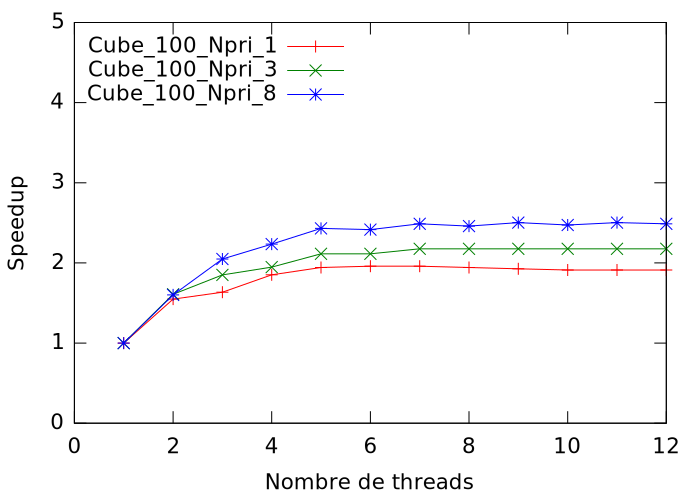
\includegraphics[width=0.7\textwidth]{res_spmv_omp}
  \caption{Accélération du produit matrice vecteur creux sur Rostand en mémoire partagée.}
  \label{fig:res_spmv_omp_rostand}
\end{figure}

%-------------------------------
\subsection{Limitations mémoires}
Pour comprendre les résultats précédents nous devons étudier brièvement l'architecture des ordinateurs.
%
Les performances d'un ordinateur dépendent essentiellement de deux choses : le processeur et la mémoire.
%
Quand un programme souhaite lire une donnée en mémoire, il subit une pénalité mémoire.
%
Cette pénalité est la somme de deux contraintes :
\begin{itemize}
        \item la latence : la différence de temps entre la demande d'accès à la mémoire et la réception du premier octet;
        \item la bande passante : le nombre maximum d'octet par seconde que le bus peut envoyer/recevoir
\end{itemize}
%
De nos jours, les ordinateurs ont différents types de mémoires.
%
Il y a la mémoire cache, très proche des unités de calcul, elle a une faible latence (quelques cycles) mais sa taille est limité à quelques Mo.
%
Ensuite, il y a la mémoire RAM avec une latence de quelques centaines de cycles mais avec une taille de plusieurs Go.
%
Si nous regardons la structure mémoire de deux bancs NUMA de la figure~\ref{fig:numa_architecture}, on s'aperçoit que la distance physique des coeurs de calcul et de la mémoire est liée à la latence des accès mémoires.
%
Pour limiter le plus possible les pénalités mémoires, il est nécessaire que tous les coeurs de calcul utilisent la mémoire qui est la plus proche.
%
Par exemple, sur une machine à deux bancs NUMA, les accès à la mémoire du banc NUMA 2 depuis les coeurs du banc NUMA 1 coûterons plus chère que les accès à la mémoire du banc NUMA 1.

%   (-_-)   %
\begin{figure}
  \centering
  \includegraphics[width=0.8\textwidth]{numa_architecture}
  \caption{Exemple d'une architecture NUMA à deux processeurs.}
  \label{fig:numa_architecture}
\end{figure}

Un autre problème se situe au niveau de la bande passante.
%
La bande passante totale de la machine est distribuée entre chaque banc NUMA.
%
Pour exploiter efficacement la totalité de la bande passante, il faut répartir les données que l'on va utiliser sur tous les bancs mémoires.
%
Des interfaces de programmation existent pour connaître et améliorer la localité des données.
%
Il ne suffit pas de faire une répartition équitable, il faut aussi au moment de l'accès au données que tous les coeurs de calcul accède à des données différentes qui doivent se situer dans la mémoire qui leur est la plus proche.

%+++++++++++++++++++++++++++++++


%+++++++++++++++++++++++++++++++
\section{Gestion actuelle des machines NUMA}
De manière générale, quand un programme alloue de la mémoire, il reçoit un pointeur sur de la mémoire virtuelle.
%
Cette mémoire virtuelle est unique à chaque processus et est partagée entre les threads d'un même processus.
%
La relation entre la mémoire virtuelle et la mémoire physique est faite par le système d'exploitation.
%
Il est responsable de la bonne gestion de la mémoire physique.
%
Lorsqu'un processus accède à de la mémoire virtuelle qui n'a pas encore été mappée à de la mémoire physique, une faute de page est générée, on appelle ça toucher une page.
%
Cette faute est traitée par le système d'exploitation, il s'occupera de trouver une page mémoire libre dans la mémoire physique et il la fera correspondre à une adresse virtuelle.
%
Lors des accès mémoire du processus, la traduction de l'adresse virtuelle vers l'adresse physique est faite par un des composants du processeur, l'unité de gestion mémoire ou MMU\footnote{Memory Management Unit}.
%
De cette façon, le processus ne voit que l'espace d'adressage virtuel et ne connaît rien de l'espace d'adressage physique.
%
Le système d'exploitation peut donc changer l'emplacement physique d'une page sans affecter le fonctionnement du processus de manière totalement transparente.
%
Toutefois, l'emplacement physique d'une page virtuelle peut impacter les performances du processus sur les architectures NUMA.
%
Cet impact dépendra des connexions entre le banc mémoire physique où se situe la page et le coeur de calcul qui fait tourner le processus.

Sur une machine NUMA, lorsqu'une faute de page arrive, le système d'exploitation doit choisir sur quel banc NUMA il placera la page.
%
Avec Linux, il y a au moins trois politiques d'allocations de disponibles :
\begin{itemize}
        \item {\em First Touch}: La mémoire est allouée sur le banc NUMA du coeur de calcul qui y accède en premier.
                         Il s'agit de la politique par défaut.
        \item {\em Bind}: La mémoire est allouée sur banc NUMA spécifié en paramètre.
        \item {\em Interleaved}: Les allocations mémoires sont entrelacées parmi tous les bancs NUMA disponibles.
\end{itemize}
Sur Linux, ces politiques peuvent être choisies avec l'appel système {\em mbind}, ou avec l'outil en ligne de commande {\em numactl}.
%
La version 3.13 de Linux apporte un nouveau mécanisme de gestion de la mémoire sur les machines NUMA, il s'agit d'AutoNUMA.
%
Ce mécanisme a pour but d'optimiser le placement des pages NUMA tout long de l'exécution d'un processus (voir section~\ref{sec:autonuma}).

D'autres systèmes d'exploitation peuvent avoir leurs propres ensembles de politiques d'allocations NUMA.
%
Solaris, par exemple, fournit aussi la politique {\em next-touch}~\cite{next_touch}.
%
Avec cette politique, les pages mémoires physiques seront déplacées près du prochain coeur de calcul qui y accédera (voir section~\ref{sec:next_touch}).
%
De nombreuses bibliothèques proposent des interfaces de programmation permettant d'abstraire le placement des pages lors d'une allocation mémoire.
%
Par exemple, la libNUMA\cite{libnuma} va abstraire les appels systèmes Linux.
%
Il existe aussi des bibliothèques qui ajouteront de nouvelles politiques d'allocations ainsi que des allocations 2D optimisées\cite{minas}.

%-------------------------------
\subsection{First touch}
La politique d'allocation mémoire par défaut sous Linux s'appelle {\em First Touch}.
%
La traduction littéral serait le {\em premier toucher}, ce nom se réfère au fait qu'avec cette allocation le noyau associe une nouvelle page physique à une page virtuelle qu'à partir de la première utilisation de cette page.
%
La page physique sera choisi avec comme priorité de prendre une page dans la mémoire la plus proche du thread qui souhaite utiliser cette page.
%
L'idée derrière cette allocation n'est pas mauvaise, dans le cas d'un processus mono-thread dont l'affinité processeur est fixée à un banc mémoire, la localité mémoire sera toujours optimale.
%
Dans le cas d'un processus multi-threads dont les threads ont une affinité fixe, s'ils allouent eux-mêmes leurs mémoires et ne font quasiment aucun partage entre eux, cette allocation fonctionne toujours.
%
Mais tous les programmes ne sont pas écrits pour fonctionner de cette façon.
%
Imaginons un programme qui soit écrit pour avoir une phase d'initialisation séquentielle, avec toutes les allocations dont il aura besoin dans cette phase, alors toute la mémoire physique sera allouée sur un seul banc NUMA.
%
Il existe d'autres cas où ce type d'allocation ne permet pas d'obtenir le maximum de bande passante mémoire de la machine.
%
Par exemple dans le cas d'une application multi-processus dont tous les processus ont une affinité processeur identique et fixée à un seul banc NUMA.
%
Seulement une partie de la bande passante mémoire sera utilisée.
%
Il y a aussi le cas où les processus ont une affinité processeur leurs permettant d'utiliser n'importe quel coeur de la machine.
%
L'allocation des pages mémoires peut se faire sur un banc NUMA, puis le noyau décide de changer le processus de banc NUMA, et tous les calculs sont faits avec une mauvaise localité mémoire.
%
De plus, si le thread de calcul change souvent de coeur de calcul, l'utilisation des caches de faibles niveaux (L1 et L2) ne sera pas optimal.
%
Il est donc important de toujours fixer l'affinité processeur d'un thread à un coeur de calcul.
%
Dans notre programme, l'initialisation des données est séquentielle, donc avec une politique d'allocation first touch, toutes les données se retrouvent sur un seul banc NUMA.
%
Nous avons donc plusieurs choix pour distribuer les données :
\begin{itemize}
  \item soit nous réécrivons la partie initialisation pour qu'elle soit faite en parallèle;
  \item soit nous essayons une autre politique d'allocation qui correspond mieux à notre problème.
\end{itemize}
%
La première solution est compliquée à mettre en oeuvre et pourrait introduire de nouveaux bogues dans le code.
%
La deuxième solution nécessite moins de changement, nous avons donc essayé cette solution.

%-------------------------------
\subsection{Interleaved memory}
First touch n'étant pas parfait, il est nécessaire d'avoir d'autres politiques d'allocation.
%
La politique {\em Interleaved memory} distribue uniformément les pages mémoires sur tous les bancs mémoires en mode tourniquet.
%
Cette distribution est faite par le noyau du système d'exploitation au moment où une page mémoire est utilisée pour la première fois par le programme.
%
Sur un système d'exploitation utilisant Linux comme noyau, il suffit d'utiliser la commande {\em numactl --interleave=all ./programme} pour utiliser cette politique d'allocation dans tout le programme.
%
En plus d'avoir très peu d'impact sur le code source d'une application, la politique d'entrelacement mémoire montre des atténuations des effets NUMA dans le cas général.
%
En moyenne, il n'y a pas d'amélioration de la latence, mais la bande passante est améliorée grâce à l'utilisation simultanée de tous les liens mémoires par rapport à une initialisation séquentielle avec une politique first touch.
%
Ainsi, il est généralement intéressant d'expérimenter cette politique, avant d'étudier la question des optimisations NUMA.
%
Dans notre cas, cette politique nous donnait de meilleurs performances que la politique first touch.
%
Mais les résultats n'étaient pas suffisant.

%-------------------------------
\subsection{Next touch}
\label{sec:next_touch}
L'idée du First touch n'est pas mauvaise, mais elle impose une phase d'initialisation parallèle.
%
Au lieu de récrire toute l'initialisation d'un programme, il pourrait être intéressant d'utiliser les phases de calculs pour distribuer la mémoire sur tous les bancs NUMA.
%
C'est pour cela que la politique d'allocation {\em Next touch} a été créée.
%
Le programmeur choisit un ensemble de pages mémoires qu'il pense mal placées et définit une politique d'allocation next touch sur ces pages.
%
Lors du prochain accès mémoire à l'une de ces pages, le noyau s'occupera, si besoin, de déplacer la page mémoire vers le banc NUMA le plus proche du processeur faisant cet accès.
%
Ainsi nous pouvons obtenir une amélioration de la localité mémoire sans avoir à récrire certaines parties du code.
%
Cette politique aurait pu apporter des performances supplémentaires à notre code, mais n'étant pas disponible dans le noyau Linux, malgré des propositions d'extensions~\cite{next_touch_linux,GoFu09Next-touch}, nous n'avons pas pu l'utiliser telle quelle.
%
\`A la place, nous avons implémenté une solution similaire qui consiste à choisir manuellement l'emplacement des pages mémoires.

%-------------------------------
\subsection{AutoNUMA}
\label{sec:autonuma}
Linux n'a pas adopté la politique d'allocation Next touch.
%
\`A la place, les développeurs de Linux ont choisi d'implémenter un autre mécanisme pour améliorer la localité NUMA : {\em AutoNUMA}.
%
Ce mécanisme va analyser périodiquement une portion de la mémoire d'un processus, et de la même façon que la politique next touch, le prochain accès à une page de cette portion entrainera un déplacement de la page.
%
Pour détecter l'accès à une page, le noyau utilise la MMU.
%
Il supprime la relation adresse virtuelle vers adresse physique de la MMU et peut ainsi recevoir un signal lors du prochain accès.
%
Ce mécanisme à un surcoût, c'est pourquoi il n'est pas appliqué sur toute la mémoire d'un coup.
%
Le noyau donne la possibilité de modifier plusieurs paramètres de ce mécanisme, mais ces paramètres sont globaux.
%
Parmi ces paramètres, il y a {\em scan\_delay} et {\em scan\_size}.
%
Tous les ``scan\_delay'', les ``scan\_size'' pages suivantes sont traitées.
%
Une fois arrivé au bout de l'espace d'adressage, le scanner recommence au début de l'espace d'adressage.
%
La variable scan\_delay change de valeur en fonction du nombre de pages déplacées.
%
Elle diminue quand il y a beaucoup de fautes NUMA et augmente quand les pages sont bien placées.
%
Ainsi, une application dont les threads accèdent toujours à la même mémoire aura automatiquement un bon placement mémoire.

Ce mécanisme comporte plusieurs défauts.
%
Sa configuration est globale au système, on ne peut pas l'activer que pour un processus particulier.
%
Les paramètres ne peuvent être définis que par l'administrateur de la machine.
%
Le mécanisme s'applique sur toute la mémoire, même les zones mémoire peu utilisées.
%
Dans le cas de notre application, cette politique permet d'améliorer la localité mémoire sans changer une ligne de code.
%
Mais le surcoût lié à l'analyse du placement des pages mémoires peut devenir problématique.

%-------------------------------
\subsection{Un processus MPI par banc NUMA}
Une bonne façon de traiter les effets NUMA est de la cacher.
%
En utilisant un processus MPI par banc NUMA et une politique d'allocation first touch ou bind, on se retrouve toujours avec des accès mémoires du banc mémoire le plus proche.
%
Mais la problématique reste similaire à la problématique du choix entre la parallélisation en mémoire distribuée et la parallélisation en mémoire partagée, ce n'est pas toujours possible ou performant.
%
Dans le cas où les algorithmes en mémoire distribuée ne passent pas à l'échelle, il est nécessaire de noter que l'utilisation de cette solution multipliera par le nombre de bancs NUMA le nombre de processus MPI.

%+++++++++++++++++++++++++++++++



%+++++++++++++++++++++++++++++++
\section{Gérer le NUMA directement dans l'ordonnanceur}
%-------------------------------
\subsection{Statuts des ordonnanceurs actuels}
La gestion du placement des pages mémoires n'est pas utile si le code qui utilisera ces données ne s'exécute pas sur le bon banc NUMA.
%
Dans le cas de la programmation par tâche, chaque tâche doit connaître le banc NUMA qui lui est le plus favorable.
%
Cette information pourra être ensuite donnée à l'ordonnanceur de tâches qui s'occupera de placer correctement la tâche.
%
Actuellement, certains ordonnanceurs ont un contrôle total de la mémoire utilisée par les tâches, ils pourraient donc optimiser l'affinité NUMA des programmes, mais ils sont très peu à le faire.


PaRSEC est un cadriciel de parallélisation par tâche qui fonctionne aussi en mémoire distribuée.
%
Il est l'un des seuls ordonnanceurs à offrir un réel support des architectures NUMA.
%
Par contre son support est une analogie avec la programmation en mémoire distribuée.
%
En effet, le support du NUMA est fait avec les structures Virtual Process (VP) de PaRSEC, ce qui peut correspondre à avoir un processus MPI par banc NUMA.
%
Mais ce n'est pas si grave, le vol de tâche entre VP existe.
%
Il conserve donc l'aspect équilibrage de charge des solutions multithreadées.
%
Par contre, cette solution ne convient toujours pas à résoudre notre problème, nous essayons d'avoir le moins possible de parallélisme en mémoire distribuée.


Il existe aussi de nombreuses tentatives d'ajout du support de la localité des données à OpenMP\cite{openmp_numa}.
%
Parmi celles-ci, il y a ForestGOMP\cite{Bro10Thesis} qui propose de répartir la mémoire dès l'allocation et de placer les threads au plus près de la mémoire.

%-------------------------------
\subsection{NATaS : ordonnancer des tâches sur une machine NUMA}
Ne trouvant pas de solution adaptée à notre besoin, nous avons créer notre propre ordonnanceur de tâches.
%
Celui-ci est très basique, il ne prend en compte que l'affinité mémoire des tâches.
%
Pour cela, nous utilisons un container de tâches thread-safe par banc NUMA.
%
Ce container permet à plusieurs threads d'insérer/retirer des tâches en limitant la contention.
%
Le vol de tâche entre container a aussi été implémenter, il existe une option par tâche pour autoriser ou non le vol de tâche.
%
Dans le cas du parallélisme de boucle, une option permettant de donner une tâche spécifiquement à un thread a été implémentée.


NATas fourni aussi une api permettant de gérer les allocations mémoires et leurs placements.
%
Il permet de faire différents types d'allocations tel que :
\begin{itemize}
  \item distribuer régulièrement la mémoire;
  \item entrelacer les pages mémoires;
  \item bind memory pages.
\end{itemize}
%
Ces allocations font miroir au différent type d'ordonnancements.
%
Dans le cas d'un parallélisme de boucle avec un distribution statique, on distribura la mémoire régulièrement.
%
Dans le cas d'un graphe de tâche, le programmeur donnera la position souhaitée des tâches.
%
Il lui suffira de simuler l'exécution du code, de désactiver le vol de tâches et d'appeler la fonction de migration des pages dans chaque tâche.



NATaS s'interface avec Taggre pour améliorer les performances sur des machines NUMA.
%
La connaissance complète du graphe de tâche permet des améliorations notables sur la distribution mémoire.
%
Comme le graphe sera déroulé de haut en bas lors de son exécution, il parait naturel de distribuer les tâches par hauteur.
%
En supposant que les tâches produisent des données et que ces données sont passées en paramètre aux tâches successeurs dans le graphe, on peut essayer d'optimiser le placement NUMA.
%
Dans un premier temps, on va équilibrer la distribution des tâches sur les bancs NUMA en attribuant une affinité NUMA aux tâches.
%
Cette affinité sera choisie en fonction de la hauteur de la tâche dans le graphe et des affinités NUMA de ses prédécesseurs.
%
Le but étant d'avoir à hauteur fixée, un nombre égale de tâche par banc NUMA tout en minimisant les accès en lecture distant.



%   (-_-)   %
\begin{figure}[t!]
  \centering
  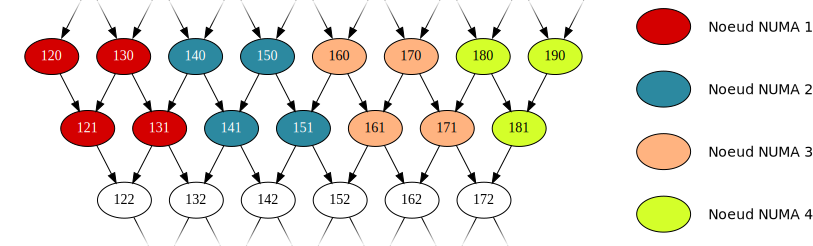
\includegraphics[width=\textwidth]{numa_distrib_example}
  \caption{Exemple de l'algorithme de distribution des tâches en action, la couleur des tâches détermine leurs affinités NUMA. Les tâches en blanches ne sont pas encore traitées.}
  \label{fig:numa_distrib_example}
\end{figure}

%+++++++++++++++++++++++++++++++


%+++++++++++++++++++++++++++++++
\section{Résultats}
%-------------------------------
\subsection{Factorisation et résolution triangulaire}
La factorisation ainsi que la résolution triangulaire utilisent le même graphe de tâches.
%
Les pages mémoires utilisées composants la matrice sont distribuée en respectant l'affinité mémoire des tâches associées.
%
Cette affinité est fournit par Taggre et correspond à une distribution à peu près équitable des pages mémoires au fil du déroulement du graphe.
%
Malheureusement, nous ne pouvons pas distribuer toutes les pages de manières optimal car il arrive que certaines pages soit utilisées par plusieurs tâches ayant des affinités mémoires différentes.
%
Dans un tel cas, nous choisissons de placer la page mémoire sur le banc NUMA ayant le plus de tâches.




\subsubsection{First touch}
Les résultats de la factorisation et de la résolution triangulaire avec une allocation first touch sont exposés dans le chapitre précèdent.
%
Les résultats ne sont pas aussi bons que ceux que nous pourrions obtenir avec une meilleure gestion de la mémoire.
%

%-------------------------------
\subsection{Multiplication matrice vecteur creuse}
La multiplication du matrice creuse par un vecteur est une opération dont le ratio nombre d'opérations par le nombre d'octet lus est petit.
%
Dans le cas d'une matrice scalaire, ce ratio vaut environ $1/10$ en double précision.
%
Pour chaque valeur non-nulles de la matrice, il faut lire cette valeur, l'indice de la colonne et la valeur contenue dans le vecteur à l'indice de la colonne.
%
Il faut ensuite multiplier les deux valeurs ensemble et l'ajouter à un accumulateur, ce qui fait en double précision 2 opérations pour 20 octets lus.
%
Si nous utilisons trois variables primaires, chaque entrée de la matrice est un bloc 3 par 3.
%
Nous devons donc lire ce bloc (9*8 Octets), lire l'indice de colonne (4 Octets) et finalement lire 3 valeurs dans le vecteur (3*8 Octets).
%
Pour chaque valeurs du bloc nous avons 2 opérations à faire (2*9), nous avons donc un ratio de $18/100$ soit environ $1/5,5$.
%
Avec huit variables primaires, le ratio monte à environ de $1/4,5$.


Le {\em roofline model} est un modèle de performance permettant de connaître la puissance de calcul maximale pouvant être atteinte par un algorithme sur une machine.
%
Ce modèle se construit de la façon suivante, dans un premier temps nous allons mesurer la bande passante maximale de la machine.
%
Pour cela nous avons utiliser le benchmark STREAM, sur Rostand, nous obtenons une bande passante de 21~Go/s.
%
Puis, dans un second temps, nous allons calculer la capacité de calcul maximale de la machine.
%
Pour calculer cette capacité, il faut multiplier le nombre de coeur de calcul par le nombre maximal d'opérations faites dans une instruction et multiplier le tout pas la fréquence d'horloge.
%
Chaque noeud de Rostand étant composé de 12 coeurs cadencés à 2,80~GHz et de l'instruction SSE~4.2 permettant d'effectuer 4 opérations flottantes à la fois, ce qui donne 134,4~GFlops.


Une fois le roofline model construit, nous pouvons donc placer le produit matrice vecteur creux.
%
Les performances du SpMV dépend du nombre de variables primaires, nous avons donc placer sur le roofline model trois SpMV en fonction du nombre de variable primaire utilisées.
%
Ces trois points nous indique que les performances du SpMV seront limitées par la bande passante mémoire.

%   (-_-)   %
\begin{figure}[t!]
  \centering
  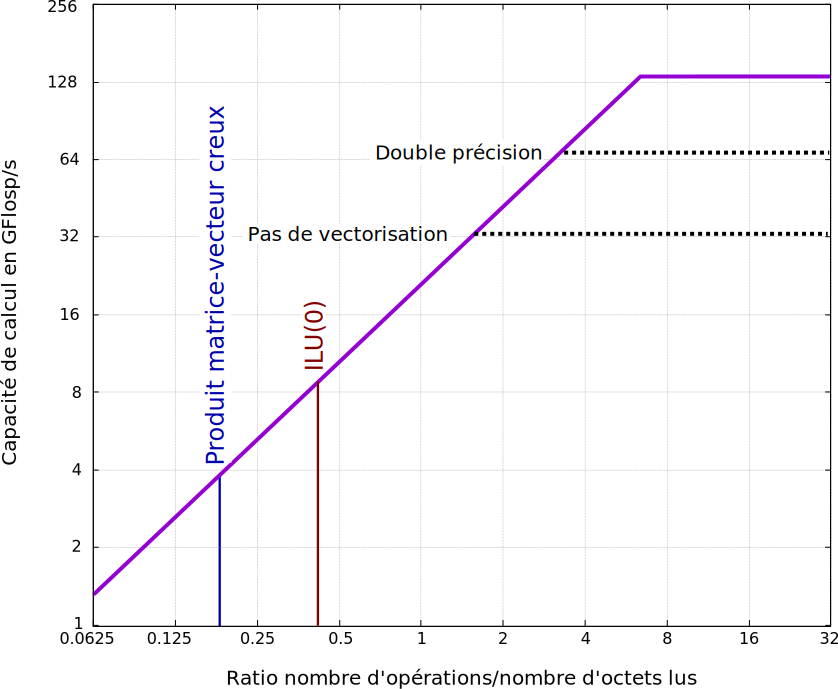
\includegraphics[width=0.8\textwidth]{roofline_rostand}
  \caption{Roofline model de Rostand. avec les différents produit matrice vecteur creux.}
  \label{fig:roofline_rostand}
\end{figure}

%-------------------------------
\subsection{First touch}
Les résultats de la factorisation et de la résolution triangulaire avec une allocation first touch sont exposés dans le chapitre précèdent.
%
Les résultats ne sont pas aussi bons que ceux que nous pourrions obtenir avec une meilleure gestion de la mémoire.
%


Le produit matrice vecteur creux ne passe pas à l'échelle.
%
Sur la machine Rostand, nous obtenons difficilement une accélération de 2,5 sur 12 coeurs en ayant 8 variables primaires (Fig.~\ref{fig:res_spmv_omp_rostand}).
%
Cette accélération descend à 1,9 en ayant 1 variable primaire, toujours sur 12 coeurs de calcul.
%
L'utilisation d'un paradigme en mémoire distribuée ne change pas le calcul mais garanti un placement mémoire optimal.
%
Les résultats sur le produit matrice vecteur sont bien meilleur qu'en mémoire partagée, nous atteignons une accélération de 3,8.
%
Cette différence est en grande partie dû aux effets NUMA, comme le montre la suite des expériences.

%   (-_-)   %
\begin{figure}[t!]
  \centering
  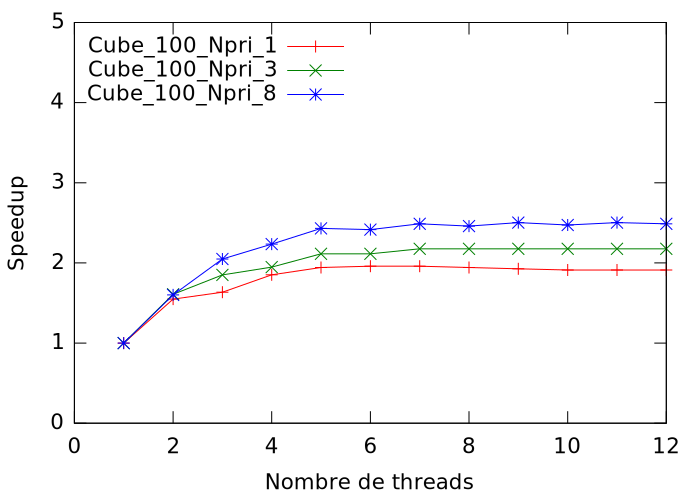
\includegraphics[width=0.7\textwidth]{res_spmv_omp}
  \caption{Accélération du produit matrice vecteur creux sur Rostand en mémoire partagée.}
  \label{fig:res_spmv_omp_rostand}
\end{figure}

%   (-_-)   %
\begin{figure}[t!]
  \centering
  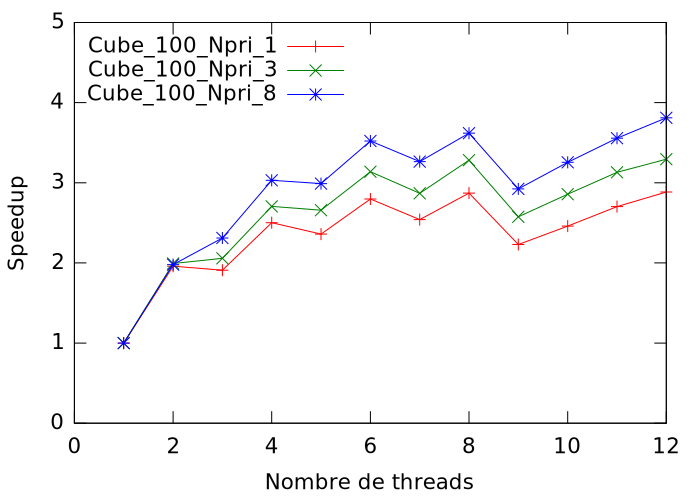
\includegraphics[width=0.7\textwidth]{res_spmv_mpi}
  \caption{Accélération du produit matrice vecteur creux sur Rostand en mémoire distribuée.}
  \label{fig:res_spmv_mpi_rostand}
\end{figure}




Sur la machine Manumanu, ces effets sont amplifiés (Fig.~\ref{fig:res_spmv_omp_manumanu}).
%
Nous obtenons les meilleurs performances en utilisant 8 coeurs avec une accélération de 5-6.
%
Utiliser plus de 8 coeurs pour effectuer le SpMV fait perdre du temps,
%
Les résultats en mémoire distribuée sont différents, les accélérations obtenues sont bien supérieures.
%
Les processus MPI sont alloués en mode compact, c'est à dire qu'ils sont distribués sur un minimum de noeud NUMA.
%
Avec 8 coeurs, nous retrouvons les même performances que la version en mémoire partagée (Fig.~\ref{fig:res_spmv_mpi_manumanu}).
%
Avec plus de processus, nous utilisons plus de noeud NUMA et nous obtenons une accélération maximal de 36.
%
En optimisant les accès mémoire de la version en mémoire partagée, nous pouvons donc espérer avoir ce même type d'accélération.


%   (-_-)   %
\begin{figure}[t!]
  \centering
  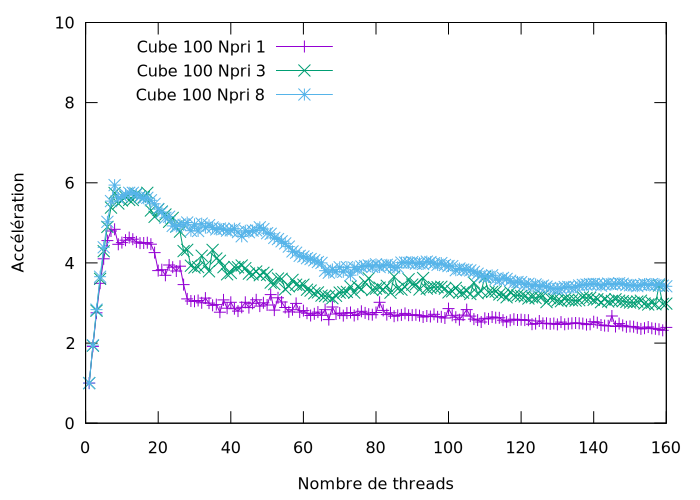
\includegraphics[width=0.7\textwidth]{res_spmv_omp_manu}
  \caption{Accélération du produit matrice vecteur creux sur Manumanu en mémoire partagée.}
  \label{fig:res_spmv_omp_manumanu}
\end{figure}

%   (-_-)   %
\begin{figure}[t!]
  \centering
  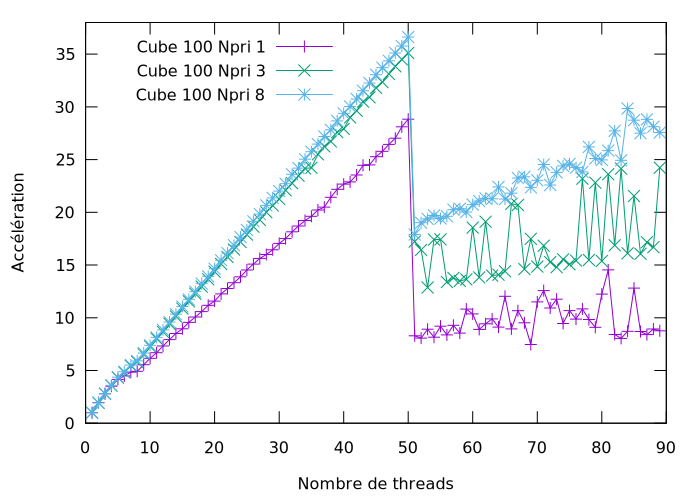
\includegraphics[width=0.7\textwidth]{res_spmv_mpi_manu}
  \caption{Accélération du produit matrice vecteur creux sur Manumanu en mémoire distribuée.}
  \label{fig:res_spmv_mpi_manumanu}
\end{figure}

%-------------------------------
\subsection{Interleave}
Pour diminuer les effets NUMA, nous pouvons utiliser la politique d'allocation interleave.
%
Cette politique va distribuer uniformément les pages mémoires sur les différents bancs NUMA.
%
Nous allons donc augmenter la bande passante mémoire en ne modifiant que légèrement la latence mémoire moyenne.
%
Sur Rostand, nous obtenons un gain de performance d'environ 20~\% mais les performances sont toujours en dessous des performances obtenues en mémoire partagée.


%% TODO résultat manumanu


%   (-_-)   %
\begin{figure}[t!]
  \centering
  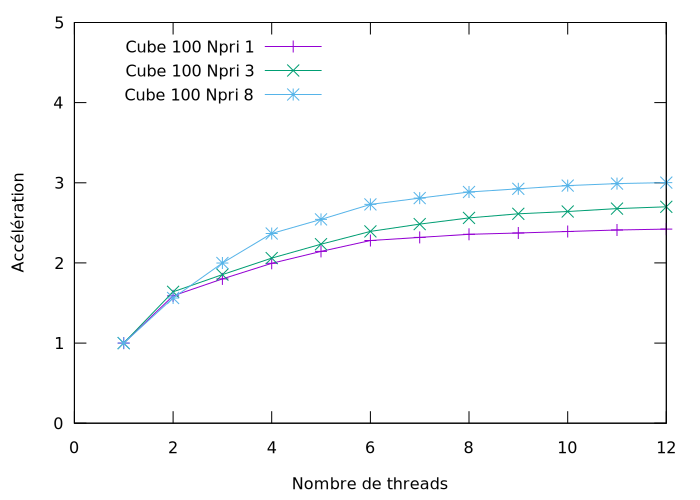
\includegraphics[width=0.7\textwidth]{res_spmv_interleave}
  \caption{Accélération du produit matrice vecteur creux sur Rostand en mémoire partagée avec une politique d'allocation interleave}
  \label{fig:res_spmv_interleave_rostand}
\end{figure}


Concernant la partie préconditionneur, l'activation de l'allocation interleave permet de gagner XX~\% de performance.
%
Regarder les compteurs matérielles.

%-------------------------------
\subsection{\'Equilibrage automatique NUMA}
Les noyaux Linux récents proposent un équilibrage de charge automatique des pages mémoires.
%
Malheureusement, nous ne pouvons pas utiliser les grappes de serveurs à notre disposition pour tester cette fonctionnalité.
%
La version de Linux disponible sur ces machines n'est pas assez récente, la fonctionnalité autoNUMA n'est apparue que dans la version 3.13 du noyau.
%
\`A la place, nous allons utiliser une machine de bureau contenant deux processeurs Intel Xeon X5660, chaque banc NUMA dispose de 6 coeurs de calculs et de 24~Go de mémoire vive.
%
La version de Linux utilisée est la 3.18.
%
Cette méthode ne fonctionne que lorsque le programme est exécuter suffisamment longtemps pour avoir le temps d'analyser toute la mémoire utilisée.
%
Nous allons donc faire varier le nombre de résolutions GMRES effectuées pour savoir à partir de quand cette méthode devient intéressante.

%-------------------------------
\subsection{NATaS}
NATas est un super bon scheduler.

%-------------------------------
\subsection{Discussion}
Les effets NUMA sont vraiment importants dans le cas d'une application limitée par la bande passante mémoire.
%
Une mauvaise distribution des pages mémoires peut conduire à une sous exploitation de la bande passante.
%
La politique d'allocation interleaved limite ce problème, on est sûr que tous les liens mémoires sont utilisés mais on n'a aucun contrôle sur l'amélioration de la localité des accès mémoire.
%
Malgré cela, on obtient un gain important de performance dans certains cas tels que le produit matrice vecteur creux et la résolution triangulaire.
%
Les politiques d'allocations du type next-touch et autoNUMA résolvent une bonne partie du problème en améliorant la localité mémoire.
%
Mais ces politiques ne nous permettent pas d'avoir un contrôle fin de l'accès aux données d'un thread.



La gestion des affinités NUMA directement dans l'ordonnanceur de tâches, nous permet de mieux répartir la charge mémoire.
%
La localité mémoire en devient optimale et une bonne distribution des tâches donnent de très bonnes performances.
%
L'utilisation d'un seul banc NUMA nous montre que l'ordonnanceur NATaS est moins bon que l'ordonnanceur Intel OpenMP.
%
Sur un nombre important de banc NUMA, NATaS ne passe pas à l'échelle.
%
Cet ordonnanceur a été écrit spécifiquement pour des machines à 2 bancs NUMA.
%
Les gains que nous observons avec l'utilisation de plusieurs bancs NUMA sont bien dus à une amélioration de la localité mémoire.


Malgré les bonnes performances que nous offrent NATaS, on pourrait se demander s'il s'agit de la meilleure solution.
%
En effet, le placement des tâches n'est pas optimal, de même que l'équilibrage de charge.
%
Avec les algorithmes actuels, il est impossible de supprimer complètement les accès distants, nous ne pouvons que les limiter.
%
Seule la solution utilisant un processus MPI par noeud NUMA permettrait de supprimer les accès distants.
%
Mais cette suppression se ferait au prix d'un algorithme moins efficace.
%
Donc une meilleure solution pourrait être d'améliorer les ordonnanceurs existants en leurs ajoutant une meilleure prise en charge des architectures NUMA.

%+++++++++++++++++++++++++++++++


%% %=========================================================
%% \chapter{The fork and join syndrome}
%% \minitoc
%% \vspace{1cm}
%% %=========================================================
%% %+++++++++++++++++++++++++++++++
%% %\section{Data dependencies}
%% %-------------------------------
%% %\subsection{Implicit dependencies}
%% %-------------------------------
%% %\subsection{Explicit dependencies}
%% %+++++++++++++++++++++++++++++++


%% %+++++++++++++++++++++++++++++++
%% \section{The fork and join syndrome}
%% %-------------------------------
%% \subsection{How to see it ?}
%%   \begin{itemize}
%%     \item Show that we have too much synchronization (Paje trace)
%%   \end{itemize}
%% %-------------------------------
%% \subsection{Domain decomposition and overlap}
%%   \begin{itemize}
%%     \item Explain what domain decomposition and overlap is
%%   \end{itemize}
%% %+++++++++++++++++++++++++++++++


%% %+++++++++++++++++++++++++++++++
%% \section{Pipeline GMRES steps}
%%   \begin{itemize}
%%     \item explain the solution to merge graph of task
%%   \end{itemize}
%% %+++++++++++++++++++++++++++++++


%% %+++++++++++++++++++++++++++++++
%% \section{Results}
%% %-------------------------------
%% \subsection{Without MPI}
%%   \begin{itemize}
%%     \item Almost no gain because no many sync
%%   \end{itemize}
%% %-------------------------------
%% \subsection{With MPI}
%%   \begin{itemize}
%%     \item Gain when increase number of MPI process
%%   \end{itemize}
%% %-------------------------------
%% \subsection{Discussion}
%% %+++++++++++++++++++++++++++++++




%=========================================================
\chapter{Conclusions and perspectives}
\minitoc
\vspace{1cm}
%=========================================================
%+++++++++++++++++++++++++++++++
\section{Conclusion}
  \begin{itemize}
    \item Coarsening allow us to parallelize problems with very small computation per task
    \item Improve bandwidth thanks to NUMA architecture
  \end{itemize}
%+++++++++++++++++++++++++++++++


%+++++++++++++++++++++++++++++++
\section{Perspectives}
  \begin{itemize}
    \item Automatic coarse tuning
  \end{itemize}
%+++++++++++++++++++++++++++++++



\backmatter % book mode only
%\bibliographystyle{alpha}
\appendix

\bibliographystyle{annotate}
\bibliography{thesis}
\end{document}
